\documentclass[reprint,prb,superscriptaddress]{revtex4-1}
\usepackage{braket,amsmath,amssymb,graphicx,float,hyperref,color,ulem,soul,lipsum}
\allowdisplaybreaks
\bibliographystyle{apsrev4-1}
\usepackage{xcolor}

%\pagecolor[rgb]{0.5,0.5,0.5}
%\color[rgb]{1,1,1}

\begin{document}


\tableofcontents

\section{Stargraph and its properties}
\subsection{Hamiltonian and wavefunctions}
\noindent As shown in the previous section, at the heart of multi channel Kondo there is a stargraph problem whic is the zero mode of the lowenergy fixed point Hamiltonian of the Multi channel Kondo. In this section our focus will be on the stargraph problem itself.
\begin{figure}[!h]
\centering
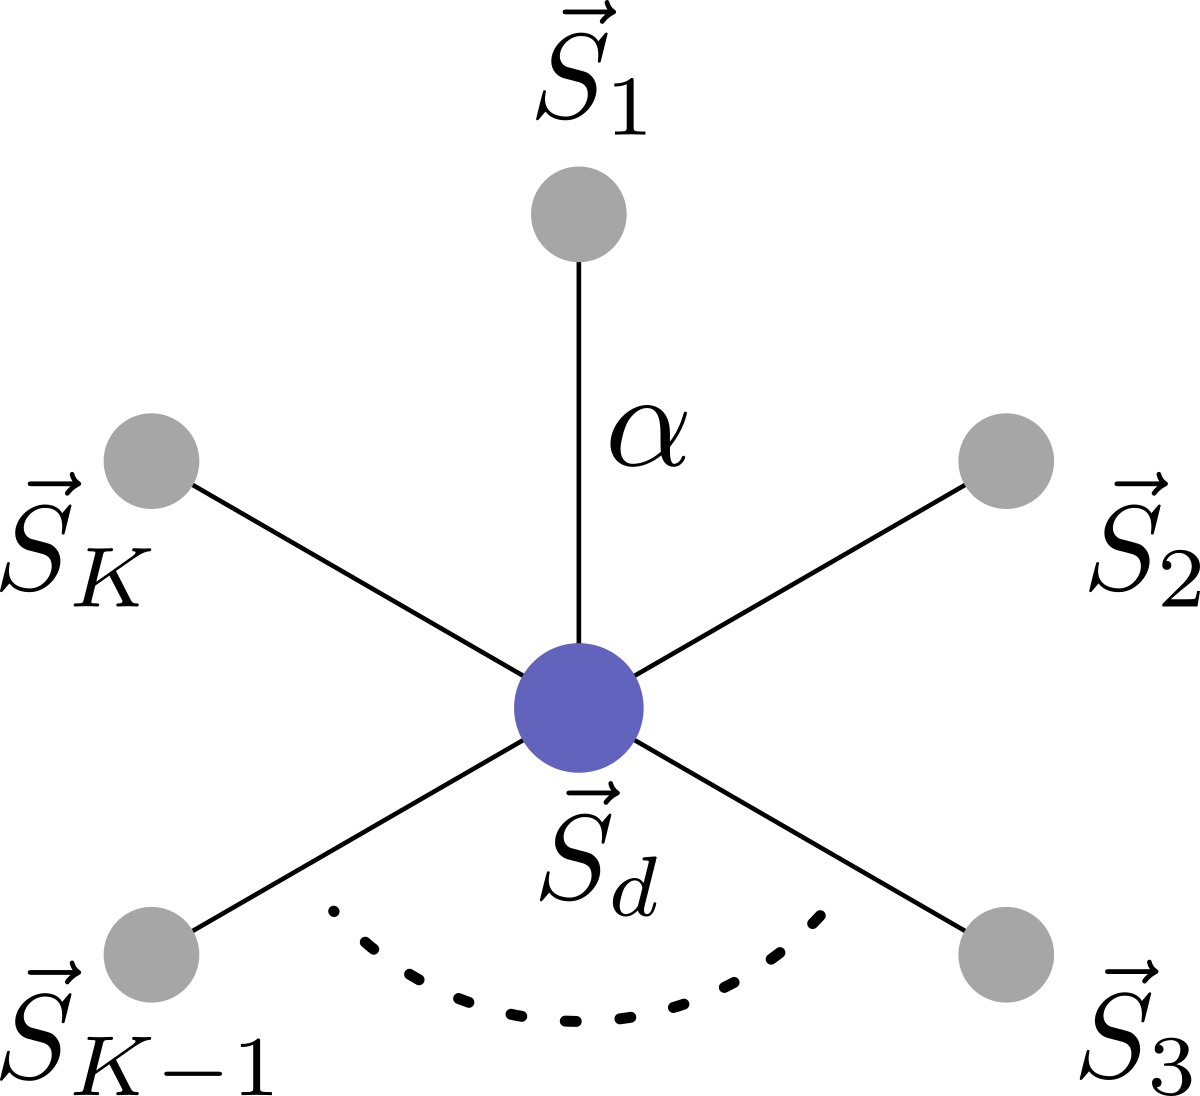
\includegraphics[scale=0.4]{plt/stargraph_first}
\caption{This is a stargraph model with one central spin $\vec{S}_d$ and $K$ outer spin $1/2$s. The central spin is coupled with all the outer spins with Heisenberg coupling with coupling strength $\alpha$.}
\label{fig:stargraph_first}
\end{figure}
As shown in the Fig.\ref{fig:stargraph_first} above one central spin ($\vec{S}_d$) is connected with $K$ spins forming a $K$ channel stargraph problem corresponding to the $K$-channel Kondo problem. The Hamiltonian of this above model is given as 
\begin{eqnarray}
H &=& \alpha \vec{S}_d.\sum_{i=1}^{K}\vec{S}_i=\alpha \vec{S}_d.\vec{S} \nonumber\\
&=& \frac{\alpha}{2} (\vec{J}^2-\vec{S}^2-\vec{S}_d^2)~,~~\alpha >0.
\end{eqnarray}
where $\vec{J}=\vec{S}+\vec{S}_d$ and $\vec{S}=\sum_{i=1}^{K} \vec{S}_i$. One can see that the large psin $S$ can take many possible values as this is made out of $K$ spin 1/2s. We can see $[H,J]=0=[H,J^i]$ for  $i=x,y,z$, $[J^i,J^j]\neq 0$ for $i\neq j$. Also the operators $\hat{Z}=2^{K+1}S_d^z\prod_{i=1}^{K} S_i^z $ and $\hat{X}=2^{K+1}S_d^x\prod_{i=1}^{K} S_i^x $ commutes with the Hamiltonian, $[H,\hat{Z}]=0=[H,\hat{X}]$ though $[\hat{Z},\hat{X}]\neq 0$, in general.
 Thus we can form the CSCO with $H,J,J^z,S,S_d$. For a particular value $S$, $J$ can take two values $S\pm S_d$ with the energies $-\alpha S_d(S_d+1\mp J)$ respectively. $S_d$ is fixed thus the energy values only depends on the corresponding $J$ value of the state. As the energy does not depends on the $J^z$, all $2J+1$ $J^z$ states labeled by $|S_d,S;J,J^z\rangle$ are degenerate. It is easy to see that the ground state has energy $E=-\alpha S_d(S_d+1+J)$ with  $J=S-S_d$, thus $E_g=-\alpha S_d(S_{max}+1)$ with $S$ taking the maximum possible value $S_{max}=K/2$.


\subsubsection{Ground state wavefunction}
\noindent Above calculations show stargraph with $K$ channels has $K$-fold ground state degeneracy, states labeled as $|S_d,S;J,J^z\rangle$ where $J^z$ takes $K=2J+1$ distinct values, $J^z=\{-J,\cdots,+J \}$. Here our goal is to find the wavefunction in the fundamental spin basis $|S_d^z,S_1^z,\cdots,S_K^z\rangle$. To achieve that we use the Clebsch-gordon coefficients, we know for two spins $j_1$ and $j_2$  with total spin $J$ and $J^z=M$ one can expand the state as 
\begin{eqnarray}
|j_1,j_2;J,M\rangle &=& \displaystyle\sum_{\substack{m_1=\{-j_1,\cdots,j_1\} \\ m_2=\{-j_2,\cdots,j_2\} }}   \mathcal{C}^{j_1,m_1;j_2,m_2}_{j_1,j_2;J,M} |j_1,m_1;j_2,m_2 \rangle ,~~~~
\end{eqnarray}
where $j_1^z=m_1$ and $j_2^z=m_2$ and $\mathcal{C}^{j_1,m_1;j_2,m_2}_{j_1,j_2;J,M}$ is the Clebs-Gordon coefficient. In our problem two spins $S_d$ and $S$ are forming one large spin $J$ represented by the state $|S_d,S;J,J^z\rangle$, in the ground state $J=S-1/2$. Thus the ground state $|S_d,S; (S-\frac{1}{2} ),M\rangle \equiv |\alpha\rangle$ can be expanded as
%{%\tiny
\begin{eqnarray}
%&&\bigg|S_d,S;\bigg(S-\frac{1}{2}\bigg),M\bigg\rangle = ww\\
&&|\alpha\rangle= \displaystyle\sum_{\substack{m_1=\{-S_d,\cdots,S_d\} \\ m_2=\{-S,\cdots,S\} }} \mathcal{C}^{S_d,m_1;S,m_2}_{S_d,S;J,M} ~~   | S_d,m_1 \rangle \otimes  |S,m_2  \rangle ,~~~~
\end{eqnarray}
%}
Because in the ground state $S$ is maximum, the state $|S,S^z\rangle$ can be decomposed in terms of a two spin problem of spin $1/2$ and $S-1/2$ forming the state $|1/2,S-1/2;S,S^z\rangle$ which can be further expanded in the basis $ |1/2,m'_1 \rangle \otimes  |S-1/2,m'_2  \rangle $ where $m'_1,m'_2$ are the z-components of the spin $1/2$ and $S-1/2$. Next we decompose the state $|S-1/2,m'_2\rangle$ in further smaller spin problem and so on. This way we finally arrive at the ground state wavefunction in terms of the fundamental basis $|S_d^z,S_1^z,\cdots,S_K^z\rangle$, give as
\begin{eqnarray}
|S_d,S;J,M\rangle &=& \sum_{S_d^z,\{S_i^z\}} \mathcal{D}_{S_d^z,\{S_i^z\}} |S_d^z,S_1^z,\cdots,S_K^z\rangle
\end{eqnarray}
where $\{S_i^z\}\equiv(S_1^z,\cdots,S_K^z)$ and the coefficient $\mathcal{D}_{S_d^z,\{S_i^z\}}$ is given as 
\begin{eqnarray}
\mathcal{D}_{S_d^z,\{S_i^z\}}  &=& \displaystyle\sum_{\substack{m_2=[-S,S]\\ m_4=[-(S-1/2),(S-1/2)]\\~.~\\  m_{2N-4}=[-1,1]   }} \mathcal{M}^{S_d^z,S_1^z,~.~.~ ,S_K^z}_{m_2,m_4,~.~.~ ,m_{2N-2}}~,~~~~~~
\end{eqnarray}
and further the coefficients $\mathcal{M}^{S_d^z,S_1^z,~.~.~ ,S_K^z}_{m_2,m_4,~.~.~, m_{2N-2}} \equiv\Sigma$, are made out of the products of Clebsh-Gordon Coefficients
\begin{eqnarray}
%\mathcal{M}^{\{m^{(1)}\}}_{\{m^{(2)}\}} &=& 
\Sigma=\mathcal{C}^{S_d,S_d^z;S,m_2}_{S_d,S;J,M} ~~ \mathcal{C}^{S_1,S_1^z;(S-1/2),m_4}_{S_1,(S-1/2);S,m_2} \cdots  \mathcal{C}^{S_{K-1},S_{K-1}^z;S_K,S_K^z}_{S_{K-1},S_{K};1,m_{2N-4}}~,~~~~
\end{eqnarray}
Using these wavefunctions we can calculate various entanglement features of this stargraph problem.


\subsection{Entanglement properties}
\noindent Using the above exact wavefunctions we can numerically compute various entanglement properties of this stargraph model. 

\subsubsection{Impurity entanglement entropy}
\noindent Here we are interested in finding the entanglement of the central impurity spin with the rest of the multi-channel bath zero mode. We know that for multi channel case the ground state is degenerate, thus for each degenerate state we can calculate the entanglement entropy. As we have already discussed for $N_{ch}$ number of channels there are $N_{ch}$ number of degenerate ground states, labeled by the $J_z$ quantum number.\\
\par For single channel case the the ground state is unique and is 
\begin{eqnarray}
|J=0,J_z=0 \rangle &=& \frac{1}{\sqrt{2}} (|\uparrow_{d}\downarrow_0\rangle -|\downarrow_d \uparrow_0\rangle)
\end{eqnarray}
Thus, one can easily calculate the reduced density matrix of the impurity by tracing out the $0^{th}$ state. From that reduced denisty matrix the entanglement entropy is $\log 2$, which is maximum possible for a spin-1/2.
\par Next, we are interested in findig this entanglement entropy for the multi-channel case $N_{ch}>1$. We have generated the degenerate ground states analytically using the Clebsch-Gordon coefficients. On this wavefunctions we do various entanglement and correlation studies. We start with the ground state wavefunction, $|\psi_g\rangle_{J_z}=|1/2_{d},S;J,J_z\rangle$, starting with one of those degenerate ground states labeled by $J_z$ we calculate the density matrix.
\begin{eqnarray}
\rho_{J_z}=|\psi_g\rangle_{J_z} \langle\psi_g|_{J_z}
\end{eqnarray}

\begin{figure}[!h]
\centering
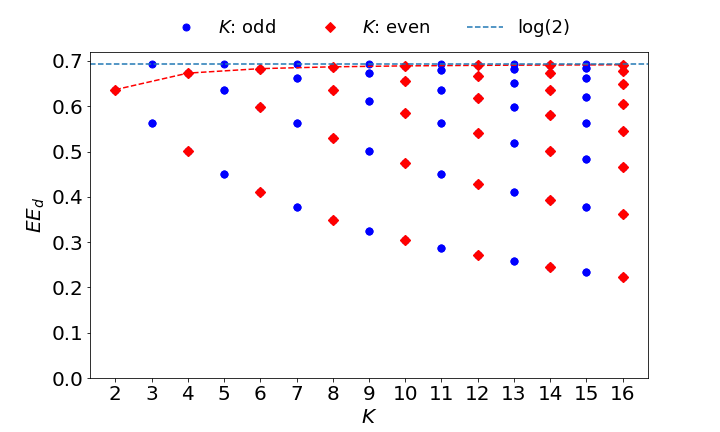
\includegraphics[scale=0.32]{plt/EE_multi_channel_ANN.png}
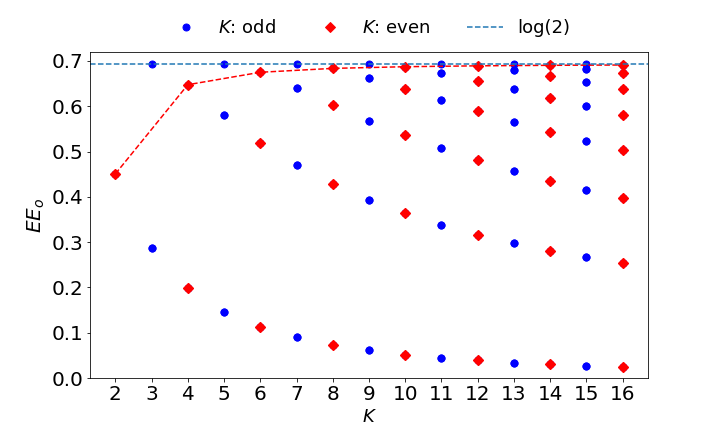
\includegraphics[scale=0.32]{plt/outer_EE_multi_channel_ANN.png}
\caption{Y-axis shows the impurity entanglement entropy with the rest and X-axis shows the number of channels $N_{ch}$. For one value of $N_{ch}>1$, there are $N_{ch}$ degenerate ground states and their corresponding impurity entanglement entropy. }
\end{figure}

\noindent Using the wavefunction we can do the partial tracing on the impurity spin to get the reduced denisty matrix of the rest. From that we get entanglement entropy for different number of channels. For even number of channel cases $J_z$ and $-J_z$ sector has same entanglement entropy. For the case of odd $N_{ch}$ there also $\pm J_z$ sectors shares same entanglement entropy, but there is a state $J_z=0$ which has entanglement entropy $\log 2$. Thus from the above we can see that $J_z=0$ state corresponding to odd number of channels shows perfect screenig interms of the maximum entanglement entropy and $J_z=0$ magnetization.


\subsubsection{Mutual Information}

Mutual information between two sub-systems $A, B$ is defined as, 
\begin{eqnarray}
I^2(A:B)=S_A+S_B-S_{A\cup B}
\end{eqnarray}

\begin{figure}[!h]
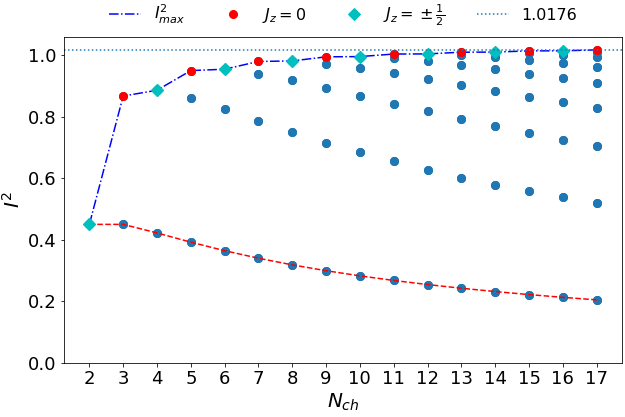
\includegraphics[scale=0.32]{plt/I_2_vs_Nch_0_1}
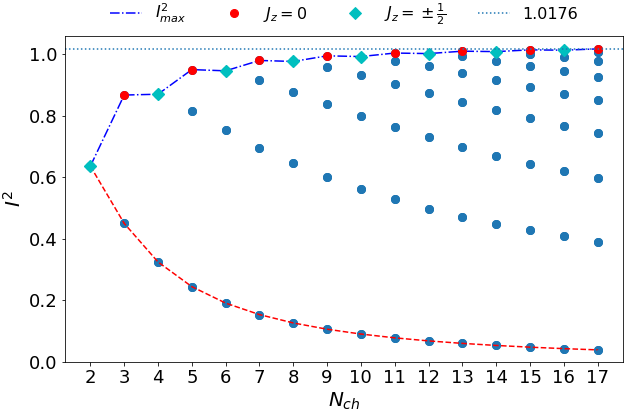
\includegraphics[scale=0.32]{plt/I_2_vs_Nch_1_2}
\caption{\textit{Left:} Y-axis is the mutual information between the impurity-spin and one outer spin and x-axis is the number of channel $N_{ch}$. \textit{Right:} This shows the variation of mutual inforamtion between two outer spins.}
\label{fig:MI_vs_Nch}
\end{figure}

We first study the mutual information between the impurity-spin and one outer spin $I^2(d:o)$. Because all the outer spins are symmetric, the mutual information between impurity-spin with any one outer spin is same. Next we calculate the mutual information between two outer spin $I^2(o:o)$. One can see that the maximum mutual information for both the cases are from the $(J_z)_{min}$ state. For odd number of channels $(J_z)_{min}=0$ and for even number of channels $\pm (J_z)_{min}=\pm 1/2$. And the minimum mutual information corresponds to the $\pm (J_z)_{max}=\pm J$ state.\\

\par As can be seen from the above Figure.\ref{fig:MI_vs_Nch} that  both the maximum mutual information of $I^2(d:o)$ and $I^2(o:o)$ try to saturate near the same value. Thus in the lowest $J_z$ sector the entanglement distribution between impurity and outer vs outer and outer is same. Which suggests that even though there were no coupling among the outer spins explicitly, there are entanglement among them. The minimum of the mutual information coming from the largest $J_z$ sector, the $I^2(o:o)$ corresponding to this sector asymptotically approach zero for large $N_{ch}$ limit. Which shows that in the large channel limit $N_{ch}\gg 1$ though the $min~I^2(o:o)$ pparoach zero the $min~ I^2(d:o)$ 

\subsubsection{Tri-partite information}
\noindent Apart from Mutual information we can calculate the tri-partie information also. This tri-partite information is defined among three sub-systems $A,B,C$ , as 

\begin{eqnarray}
I^3_{A,B,C} &=& (S_A+S_B+S_C)-(S_{AB}+S_{BC}+S_{CA})+S_{ABC}~,
\end{eqnarray}

\begin{figure}[!h]
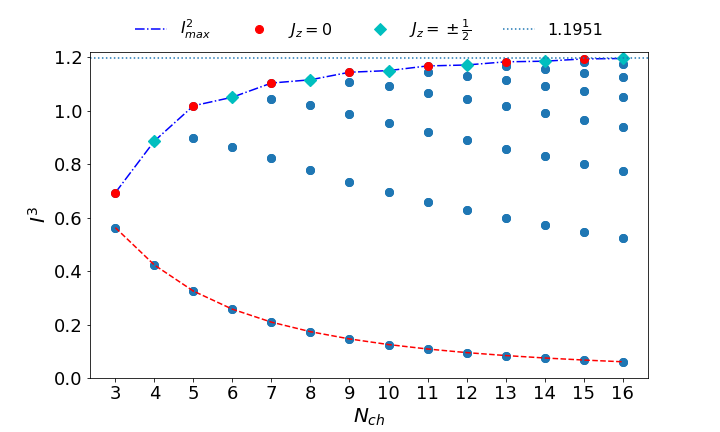
\includegraphics[scale=0.32]{plt/I_3_vs_Nch_1_2_3}
%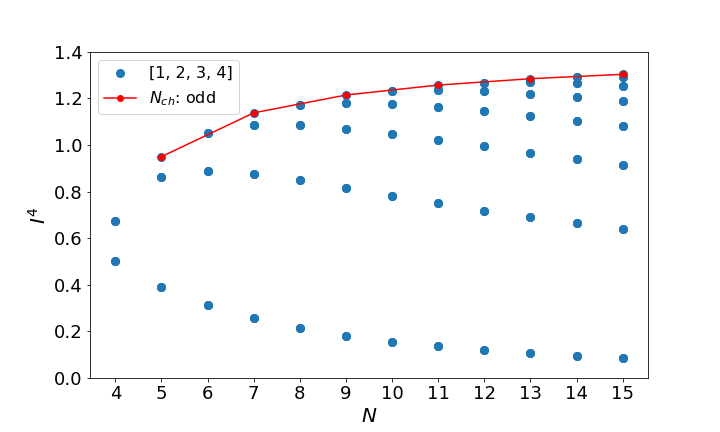
\includegraphics[scale=0.32]{plt/I_4_vs_Nch_1_2_3_4}
\caption{This plot shows the variation of the tri-partite information with the number of channels $N_{ch}$.}
\label{fig:I3_vs_Nch}
\end{figure}
\noindent Our tri-partite infrmation measure (Fig.\ref{fig:I3_vs_Nch}) among the outer spins shows that the just like the mutual information the minimum tri-partite information asymptotically approaches zero in the $N_{ch}\gg 1$ limit. Same is the case for 4-partite information also.

\subsubsection{$I_N$ vs N}
\noindent Here we are intersted in understading the entanglement dristribution among different number of outter spins. To find that out we take a multi-channel stargraph model with $N_{ch}$ noumber of outer spins. We calculate different multi partite inforamtions $I^m, m\in \{2,\cdots,N_{ch}\}$ on it's $N_{ch}$ degenerate ground states. 

\begin{figure}
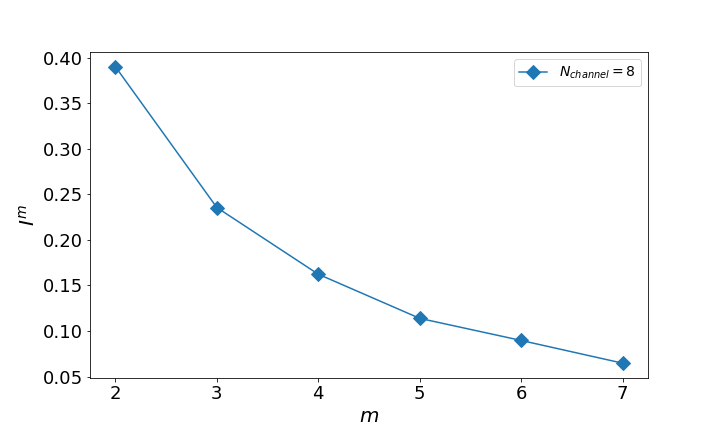
\includegraphics[scale=0.32]{plt/I_N_vs_N_N9.png}
\caption{This figure shows how the $m-partite$ information varies with $m$ showing the entanglement distribution amond different number of outer-spins.}
\label{fig:Im_vs_m}
\end{figure}
\noindent Our above study (Fig.\ref{fig:Im_vs_m}) shows that the mutual imformation has the maximum value and higher odere multi-parite informations is smaller and smaller approaching zero.

\subsection{Correlation Studies}

\subsubsection{Quantum energy}
\noindent Here we are interested in the energy expectation value arising from the quantum fluctuation part of the Hamiltonian (\ref{eq:zero_mode}). We define ising enregy $E_{ising}$ and quantum energy $E_{Q}$ in the ground state $|\psi_g\rangle$ as,
\begin{eqnarray}
E_{ising} = |\langle \psi_g | \mathcal{H}^c_0 | \psi_g \rangle| ,~~ E_{Q} &=& |\langle \psi_g | \mathcal{H}^Q_0 | \psi_g \rangle|=|E_g|-|E_{ising}|~, \nonumber\\
&=& \frac{\alpha(S+1)}{2} - |E_{ising}|.
\end{eqnarray}  
This quantum energy $E_Q$ is generated by the spin-flips between the impurity spin and the outer spin. Thus it is interesting to findout how this quantum energy changes with the increase of the number of channels $(N_{ch})$. Another important parameter is the Quantum enrgy per channel, $e_Q=|E_Q|/N_{ch}$, and it's variation towards the infinity channel limit. We know in the gorund state $N_{ch}=2S$ thus,
\begin{eqnarray}
e_Q &=& \frac{\alpha(S+1)}{4S} - \frac{|E_{ising}|}{2S} ~,~\nonumber\\
%&=& \alpha\frac{(N_{ch}+2)}{4N_{ch}}-\frac{|E_{ising}|}{N_{ch}} ~,~ \nonumber\\
%&=& \alpha \bigg(\frac{1}{4} +\frac{1}{2N_{ch}} \bigg)-\frac{|E_{ising}|}{N_{ch}}~,~\nonumber\\
&=& \frac{\alpha}{4} -\frac{1}{N_{ch}} \bigg(|E_{ising}| -\frac{\alpha}{2}  \bigg)~,~
\end{eqnarray}
Thus from the above equation of quantum energy per channel one can see that in the inifinity-channel limit $N_{ch}\rightarrow \infty$, 

\begin{eqnarray}
e_Q = \frac{\alpha}{4}- \frac{|E_{ising}|}{N_{ch}} < \frac{\alpha}{4}~,~
\end{eqnarray}

\begin{figure}[!h]
\centering
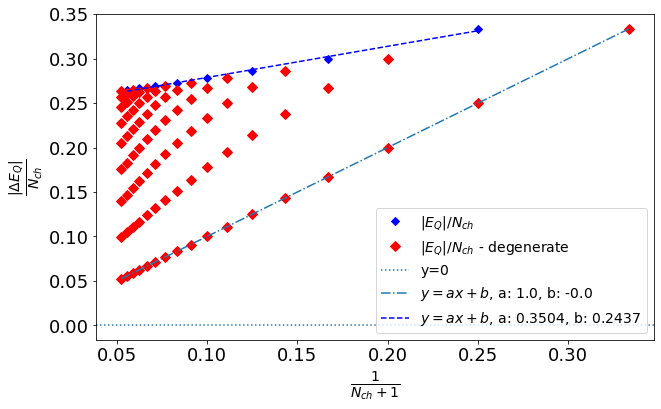
\includegraphics[scale=0.34]{plt/Quantum_Energy_per_channel}
\caption{This shows the variation of quantum energy per channel with $1/N$, where $N=N_{ch}+1$ is the total number of spins in the systems including the impurity spins. }
\end{figure}


\subsubsection{Correlation study}
Here we want to calculate various correlation functions in the ground state. We start with the expectation value of $J_z^2$ in the ground state $|\psi_g\rangle$,
\begin{eqnarray}
j_z^2&=&\frac{1}{N_{ch}}\langle \psi_g | J_z^2 | \psi_g \rangle~=\frac{1}{N_{ch}} \bigg[ J^2-(J_x^2+J_y^2) \bigg] ~,\nonumber\\
%&=& \frac{1}{N_{ch}} \bigg[ (S^2-1/4)-(J_x^2+J_y^2) \bigg] \nonumber\\
&=& \frac{1}{N_{ch}} \bigg[ \frac{(N_{ch}^2-1)}{4}-(J_x^2+J_y^2) \bigg]
\end{eqnarray}

\begin{eqnarray}
\langle \psi_g | J_{z}^2 | \psi_g \rangle_{max} &=& \bigg(\frac{N_{ch}-1}{2}\bigg)^2~,\nonumber\\
\langle \psi_g | J_{z}^2 | \psi_g \rangle_{min} = \bigg(\frac{N_{ch}-(N_{ch}-1)}{2}\bigg)^2&=&\frac{1}{4}~,~\textrm{for $N_{ch}$ even}.\nonumber\\
&=& 0 ~,~\textrm{for $N_{ch}$ odd}.
\end{eqnarray}
Thus,
\begin{eqnarray}
\langle (J_x)^2+(J_y)^2 \rangle_{max}&=&\langle J^2 \rangle - \langle J_z^2 \rangle_{min} ~,\nonumber\\
&=& \frac{N_{ch}^2-1}{4}-\frac{1}{4}=\frac{N_{ch}^2-2}{4}~, \textrm{for $N_{ch}$ even } \nonumber\\
&=& \frac{N_{ch}^2-1}{4}~, \textrm{for $N_{ch}$ odd } \nonumber
\end{eqnarray}
Which shows, for single channel case $N_{ch}=1$, this quntum fluctuation expectation value vanishes, while for multi channel this takes non-zero values. Thus 
\begin{eqnarray}
\frac{1}{N_{ch}}\langle (J_x)^2+(J_y)^2 \rangle_{max}
&=& \frac{N_{ch}}{4}-\frac{1}{2N_{ch}}  ~, \textrm{for $N_{ch}$ even } \nonumber\\
&=& \frac{N_{ch}}{4}-\frac{1}{4N_{ch}}~, \textrm{for $N_{ch}$ odd } \nonumber
\end{eqnarray}
Thus in the large channel number limit $N_{ch}\gg 1$, one can see that 
\begin{eqnarray}
\frac{1}{N_{ch}}\langle (J_x)^2+(J_y)^2 \rangle_{max}
\rightarrow \frac{N_{ch}}{4}~,~\textrm{for both even and odd $N_{ch}$}
\end{eqnarray}
\noindent $J_z$ can take values $\{-J,-J+1,\cdots,J-1,J\}$ in the ground state, where $J=S-1/2=(N_{ch}-1)/2$.




\subsubsection{Staggerred magnetization}
One can analytically check the single channel Kondo results. $N_{ch}=1$, thus here the ground state is unique.
\begin{eqnarray}
|\psi_g\rangle &=& \frac{1}{\sqrt{2}} \bigg(|\uparrow\downarrow\rangle-|\downarrow\uparrow\rangle\bigg)= |J=0,J_z=0\rangle
\end{eqnarray}
Thus in this ground state $\langle J_z \rangle=0$ and the  entanglement entropy is $\log 2$ the maximum value. Now we define a staggered magnetization (\ref{fig:st_mag}) operator $M_s$ measure,


\begin{figure}
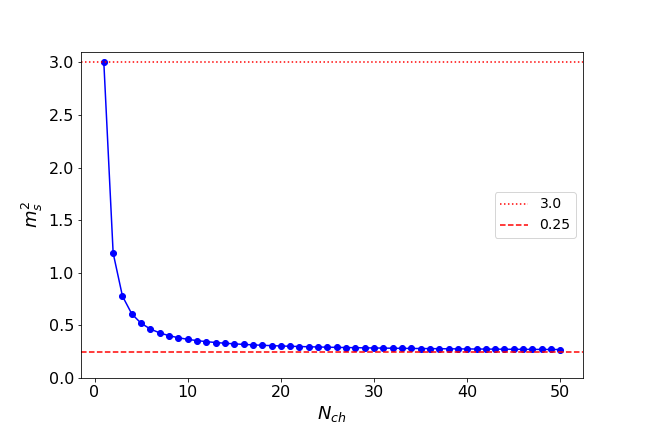
\includegraphics[scale=0.36]{plt/Staggered_mag_50.png}
\caption{This shows how the staggered magnetization changes with the number of channels $N_{ch}$.}
\label{fig:st_mag}
\end{figure}

\begin{enumerate}
\item For the single channel case both the $\vec{S}_d$ and $\vec{S}$ are spin-1/2 object and the total spin is defined as $\vec{J}=\vec{S}_d+\vec{S}$. Here $\vec{S}$ is the total outer spin.

\begin{eqnarray}
M_s^2 = \langle \psi_g | (\vec{S}_d - \vec{S})^2 |\psi_g\rangle &=& \langle \psi_g | 2(\vec{S}_d^2 + \vec{S}^2)-\vec{J}^2 |\psi_g\rangle \nonumber\\
&=& 2 \langle \psi_g | \vec{S}_d^2 +\vec{S}^2 |\psi_g\rangle \nonumber\\
&=& 3
\end{eqnarray}

\item \begin{eqnarray}
M_s^2 &=& \langle \psi_g | (\vec{S}_d - \vec{S})^2 |\psi_g\rangle = \langle \psi_g | 2(\vec{S}_d^2 + \vec{S}^2)-\vec{J}^2 |\psi_g\rangle \nonumber\\
&=&  \bigg\langle \psi_g \bigg| 2\bigg(\frac{3}{4}+ \frac{N_{ch}(N_{ch}+2)}{4}\bigg)- \frac{(N_{ch}+1)(N_{ch}-1)}{4} \bigg|\psi_g \bigg\rangle \nonumber\\
&=& \frac{N_{ch}^2}{4}+N_{ch}+\frac{7}{4}
\end{eqnarray}

\end{enumerate}

\noindent Thus, staggered magnetization squared per channel,
\begin{eqnarray}
m_s^2=\frac{M_s^2}{N_{ch}^2}=\frac{1}{4}+\frac{1}{N_{ch}}+\frac{7}{4N_{ch}^2} \xrightarrow[]{N_{ch}\gg 1} \frac{1}{4}+\frac{1}{N_{ch}}~,
\end{eqnarray}
\begin{eqnarray}
\frac{\vec{J}^2}{N_{ch}^2}&=&\frac{(\vec{S}_d+\vec{S})^2}{N_{ch}^2}= \frac{N^2_{ch}-1}{4N^2_{ch}} \xrightarrow[]{N_{ch}\gg 1} \frac{1}{4}~. \nonumber 
\end{eqnarray}

Using the $SU(2)$ property of our problem, we can define $m_s$ for each spatial direction, in 3D there are three independent spatial direction.
\begin{eqnarray}
\langle(m_s^x)^2\rangle=\langle(m_s^y)^2\rangle=\langle(m_s^z)^2\rangle=\frac{1}{3}m_s^2~,~~   
\end{eqnarray}
We define $m_Q^2=m_s^2-1/4$ which in the the large $N_{ch}$ limit becomes $1/N_{ch}$ and eventually vanishes in the $N_{ch}\rightarrow \infty$ limit. 


\noindent Thus to summarize,
\begin{enumerate}
\item In the single channel problem, $\langle (m_s^z)^2 \rangle=1$. 
\item In the multi-channel case,  
$\langle (m_s^z)^2 \rangle=\frac{1}{3N_{ch}}+\frac{1}{12}+\frac{7}{12N_{ch}^2} \xrightarrow[]{N_{ch}\gg 1} \frac{1}{12}+\frac{1}{3N_{ch}}\rightarrow \frac{1}{12}$. 
This show partial screening.
\end{enumerate}

Thus it is important to find the scaling of 

\begin{enumerate}
\item $M_s^2$ vs $N_{ch}$.
\item Uncompensated Quantum Fluctuation vs $N_{ch}$.
\end{enumerate}

\subsection{Calculating thermodynamic quantities}
We take the stargraph Hamiltonian and do the exact diagonalization and find the entire eigenspectrum. Using the full eigenspectrum we calculate the partition function $Z=\sum_i e^{-\beta E_i}$, where $E_i$ is the energy of the $i^{th}$ state. One can rewrite this partition function interms of the state degeneracies as $Z=\sum_{\epsilon} d(\epsilon) e^{-\beta \epsilon} $, where $d(\epsilon)$ is the degeneracy of the state with energy $\epsilon$. Thus the free energy is given as $\mathcal{F}=-k_BT\log Z$. 
\subsubsection{Thermal entropy}
Thermal entropy is defined as $S=-(\frac{\partial \mathcal{F}}{\partial T})_H$, where $H$ represents a constant magnetic field. In ourcase we will be interested in the zero field case. 
\begin{eqnarray}
\mathcal{F}&=& -k_B T\log Z \nonumber\\
S &=& -(\frac{\partial \mathcal{F}}{\partial T}) = -k_B \log Z -k_B T \frac{1}{Z} \frac{dZ}{dT}
\end{eqnarray}
Now 
\begin{eqnarray}
Z =\sum_\epsilon  d(\epsilon)e^{-\beta \epsilon} ~~\Rightarrow ~~  \frac{dZ}{dT} &=& \sum_\epsilon d(\epsilon) e^{-\beta \epsilon}  (-\epsilon) \frac{d\beta}{dT} \nonumber\\
&=& \sum_\epsilon d(\epsilon) e^{-\beta \epsilon}   \frac{ \epsilon}{k_B T^2} =k_B\sum_\epsilon \epsilon d(\epsilon) e^{-\beta \epsilon} \beta^2   
\end{eqnarray}
Thus we get
\begin{eqnarray}
S &=& -k_B \log \sum_{\epsilon} d(\epsilon) e^{-\beta \epsilon}  -\frac{1}{\beta} \frac{k_B\sum_\epsilon \epsilon d(\epsilon) e^{-\beta \epsilon} \beta^2   }{\sum_\epsilon  d(\epsilon)e^{-\beta \epsilon}} \nonumber\\
\lim_{\beta\rightarrow \infty} S &=& -k_B \log_2 d(\epsilon_{G})  ~~, \textrm{and}~~ \lim_{\beta\rightarrow 0} S = -k_B \log \sum_\epsilon d(\epsilon) 
\end{eqnarray}
\begin{figure}
\centering
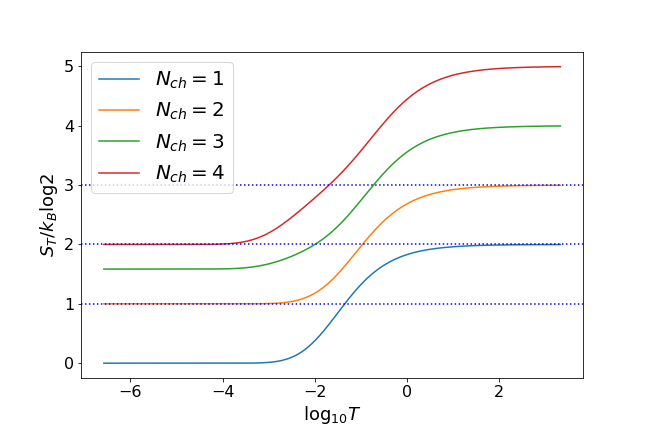
\includegraphics[scale=0.36]{plt/ThermalEntanglementVS_LogTemperature_}
\caption{This shows the variation of thermal entropy with the temperature.}
\label{fig:thermal_entropy}
\end{figure}

Thus at the extreme temperature it is easy to calculate the termal entropy, but it is difficult to visualize for any intermediate temperatures. Thus we plot the thermal entropy (unit $\log 2$) for different tempertures and for different channels in Fig.\ref{fig:thermal_entropy}. This shows at the extreme temperature the termal entropy saturates and at the intermediate temperature it changes from one to the other like a soliton like solution. At low temperature the thermal enttropy in the unit of $\log 2$ is not always quanlized but at high temperature it is. To understad this let's say at low temperature $S_T/k_B\log T=\Omega=\log_2 d(\epsilon_{G})$. Here $d(\epsilon_{G})$ is always integer and equal to the channel number $K$. Thus 
\begin{eqnarray}
d(\epsilon_{G}) &=& 2^{\Omega}=K
\end{eqnarray}
From our study we can see that for some channel number we get $S_T/k_B\log T$ tobe integer. One can easily see that those $K=2^n$ channel cases, $n$ is an integer will have integer thermal entropy. Thus between $m$ and $m+1$ integer thermal entropy plateau there will be $(2^m-1)$ number of fractional thermal entropy plateau, which is always odd.

\subsubsection{Suseptibility}
\begin{enumerate}
\item Impurity-field susceptibility : Now we add small magnetic field to the impurity spin and calculte the suseptibility as a function of temperatur for different channel cases.
\begin{figure}
\centering
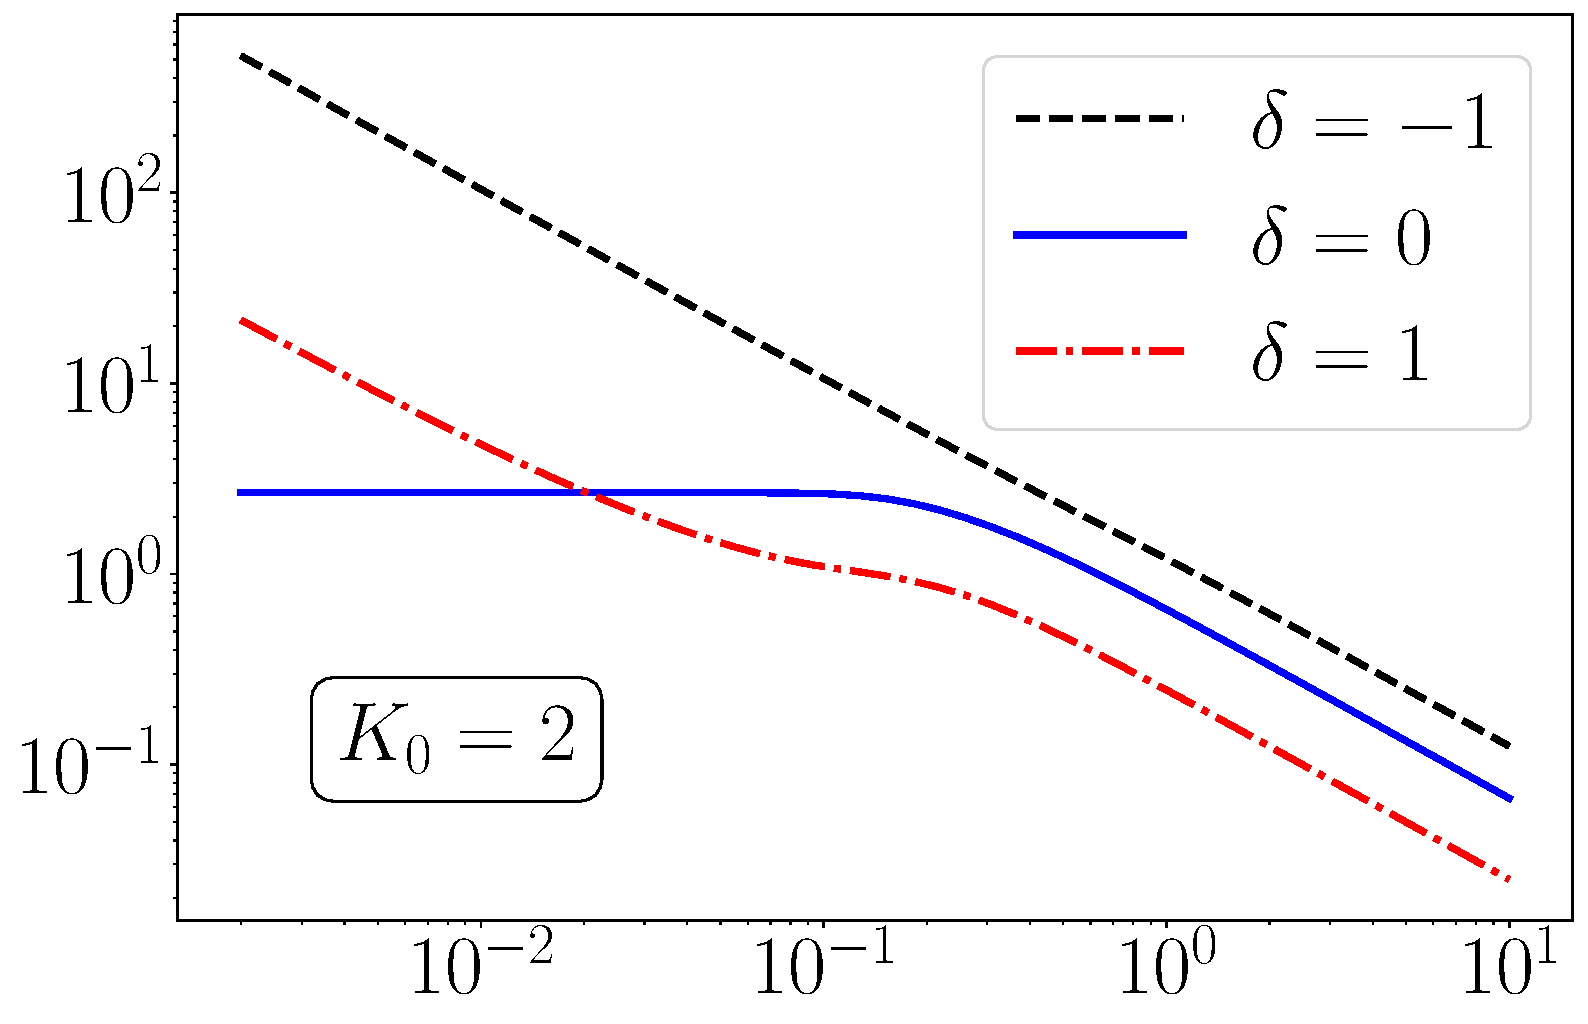
\includegraphics[scale=0.36]{plt/Central_Field_Chi_Powerlaw_}
\caption{Impurity susseptibility vs temperature.}
\label{fig:suseptibility_impurity}
\end{figure}

\item Outer-field suseptibility: Now we add a unifor magnetic field on the outer spins and calculate the suseptibility for different chanel cases.
\begin{figure}
\centering
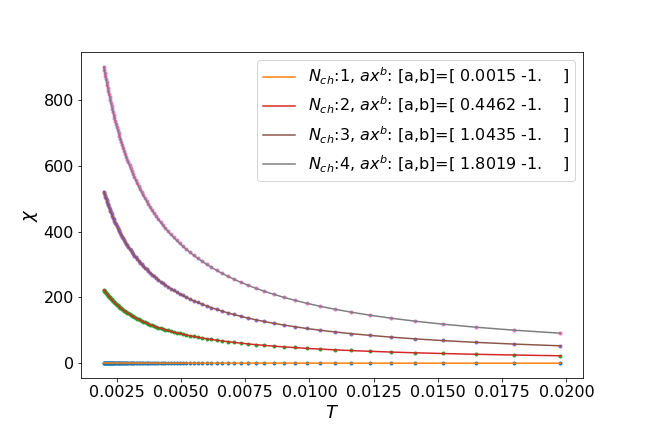
\includegraphics[scale=0.36]{plt/Outer_Field_Chi_Powerlaw_}
\caption{Outer susseptibility vs temperature.}
\label{fig:suseptibility_outer}
\end{figure}
\end{enumerate}
As can be seen from the above results that the both impurity and outer field suseptibility follows a power law in temperature for $K>1$ case. 
\begin{eqnarray}
\chi_{imp}(T) \sim T^{-1} ~,~\chi_{outer} \sim T^{-1}
\end{eqnarray}
This shows an universality among the greater than one channels.


\section{Excitation properties}
Here we start with the low energy zero mode fixed point Hamiltonian for the two-channel Kondo obtained under URG treatment. Our goal here is to add excitations on top of this ground state and using the perterbation theory. In doing so we consider the leading order scatter apprearing in the lowest order in the perturbative expansion. Note, in the fixed point zero mode Hamiltonian impurity spin is coupled with the bath electrons via spin exchange coupling, there is no charge exchange coupling present. 
\begin{eqnarray}
H^{(2)}&=& \alpha \vec{S}_{imp}.(\vec{S}_1+\vec{S}_2)~~,~~\vec{S}_i =  \frac{1}{2}~ c_{i,\alpha}^{\dagger}~ \vec{\sigma}_{\alpha,\beta}~ c_{i,\beta}
\label{eq:channel-2-spin}
\end{eqnarray}
Here $\vec{S}_i=1,2$ represents the spin degree of freedom present in the origin of the $i^{th}$ channel. Thus one can rewrite the Eq.\eqref{eq:channel-2-spin} interms of the electronic degree of freedom as,
\begin{eqnarray}
\mathcal{H}_0= H_{0_1}+H_{0_2} &=& \alpha S^z_{imp}.\bigg(\frac{n_{1,\uparrow}-n_{1,\downarrow}}{2} \bigg) + \frac{1}{2} \bigg( S_{imp}^{+} c^{\dagger}_{1,\downarrow} c_{1,\uparrow} - S_{imp}^{-} c_{1,\uparrow}^{\dagger} c_{1,\downarrow} \bigg)\nonumber\\
&& ~~~+~~ \alpha S^z_{imp}.\bigg(\frac{n_{2,\uparrow}-n_{2,\downarrow}}{2} \bigg) + \frac{1}{2} \bigg( S_{imp}^{+} c^{\dagger}_{2,\downarrow} c_{2,\uparrow} - S_{imp}^{-} c_{2,\uparrow}^{\dagger} c_{2,\downarrow} \bigg)
\end{eqnarray}
Here the basis we are interested in is $\{\mathcal{B}\}=\{|S^z_{imp},n_{1,\uparrow},n_{1,\downarrow},n_{2,\uparrow},n_{2,\downarrow}\rangle \}$. In this basis we write down all $2^3=8$ states of the spin Hamiltonian eq.\eqref{eq:channel-2-spin}
\begin{eqnarray}
|\alpha_0\rangle &=& \frac{1}{\sqrt{6}} \bigg[2|\Downarrow,1,0,1,0\rangle-|\Uparrow,0,1,1,0\rangle-|\Uparrow,1,0,0,1\rangle\bigg] \nonumber\\
|\alpha_1\rangle &=& \frac{1}{\sqrt{6}} \bigg[2|\Uparrow,0,1,0,1\rangle-|\Downarrow,1,0,0,1\rangle-|\Downarrow,0,1,1,0\rangle\bigg] \nonumber\\
&& E_{\alpha_0}= E_{\alpha_1}= -\alpha
\end{eqnarray}
\begin{eqnarray}
|\beta_0\rangle &=& \frac{1}{\sqrt{2}}\bigg[|\Downarrow,1,0,0,1\rangle-|\Downarrow,0,1,1,0\rangle \bigg] \nonumber\\
|\beta_1\rangle &=& \frac{1}{\sqrt{2}} \bigg[ |\Uparrow,1,0,0,1\rangle-|\Uparrow,0,1,1,0\rangle \bigg]\nonumber\\
&& E_{\beta_1}=E_{\beta_2}=0
\end{eqnarray}
\begin{eqnarray}
|\gamma_{0}\rangle &=&\frac{1}{\sqrt{3}} \bigg[|\Uparrow,0,1,0,1\rangle+|\Downarrow,1,0,0,1\rangle+|\Downarrow,0,1,1,0\rangle \bigg] \nonumber\\
|\gamma_{1}\rangle &=& \frac{1}{\sqrt{3}}\bigg[ |\Uparrow,1,0,0,1\rangle+|\Uparrow,0,1,1,0\rangle+|\Downarrow,1,0,1,0\rangle \bigg] \nonumber\\
|\gamma_{2}\rangle &=& |\Uparrow,1,0,1,0\rangle \nonumber\\
|\gamma_{3}\rangle &=& |\Downarrow,0,1,0,1\rangle \\
&& E_{\gamma_0}=E_{\gamma_1}=E_{\gamma_2}=E_{\gamma_3}=\frac{\alpha}{2}
\end{eqnarray}
Note this spin Hamiltonian has total $8$ states, where ground state is double degenerate with energy $-\alpha$ and the lowest exicites state with energy $0$ is also double degnerate and the second excited state with energy $\alpha/2$ is 4-fold degenerate. 
\par On top of the zero mode spin-channel interactions we want to consider the effect of the momentum space kinetic energy term $\sum_{k}\epsilon_k (n_{1,k}+n_{2,k})$. We assume identical dispersion for both the channels. Our zero mode spin Hamiltonian is written in the real space, thus it will be easier to do the perterbation theory on the real space. The fourier transformation of the momentum space kinetic energy  term leads to real space hopping term. For simplicity we will be considering the neareast neighbor hoppings between sites within each channels. The real space hopping contributino to the Hamiltonian $H_X$ with the hooping strength is 
\begin{eqnarray}
H_{X} &=& -t \displaystyle\sum_{\substack{<1,l_1> \\ <2,l_2>}} (c^{\dagger}_{1,\sigma}c_{l_1,\sigma}+c^{\dagger}_{2,\sigma}c_{l_2,\sigma}+ ~\textrm{h.c.})
\end{eqnarray}
Here $l_i$ represents the nearest site to the origin of the $i^{th}$ channel. Thus here we are interested in studying the Hamiltonian $\mathcal{H}_0+H_X$. The perterbating term $H_x$ contains scattering which takes the states of the zero mode Hamltonain out of spin-channel scattering space. Thus befor we start the perturbation theroy we must expand the basis of the zero mode Hamiltonian itself. Thus the basis which contains the nearest neighbor sites of both the channels is given as 
\begin{eqnarray}
&&\{\mathcal{B}_{extnd}\} \equiv  \{\mathcal{B}\} \otimes  \{|n_{l_1,\uparrow},n_{l_1,\downarrow},n_{l_2,\uparrow},n_{l_2,\downarrow}\rangle\} \nonumber\\
&=& \{|S^z_{imp},n_{1,\uparrow},n_{1,\downarrow},n_{2,\uparrow},n_{2,\downarrow}\rangle \otimes |n_{l_1,\uparrow},n_{l_1,\downarrow},n_{l_2,\uparrow},n_{l_2,\downarrow}\rangle\} \nonumber\\
\end{eqnarray}
Note there are $2^4=16$ elements in the subspace $\{|n_{l_1,\uparrow},n_{l_1,\downarrow},n_{l_2,\uparrow},n_{l_2,\downarrow}\rangle\}$. In the spin-channel basis $\{\mathcal{B}\}$ there $2$ degenerate ground states. Because the unpurterbed Hamiltonian $\mathcal{H}_0$ has no scattering terms outside the spin sector, in the extended basis $\{\mathcal{B}_{extnd}\}$ the total ground state deneracy becomes simply $2\times 2^4$, $32$ fold. Thus the total hamiltonian we are interested in is 
\begin{eqnarray}
\mathcal{H} &=& \frac{\alpha\hbar}{2}~ \vec{S}_d. \displaystyle\sum_{i=\{1,2\}} \displaystyle\sum_{\alpha,\beta\in\{\uparrow,\downarrow\}}c_{i\alpha}^{\dagger} \vec{\sigma}_{\alpha\beta} c_{i\alpha} -t\displaystyle\sum_{i=\{1,2\}}\displaystyle\sum_{\substack{\langle i,l_i \rangle\\ \sigma}}(c^{\dagger}_{i,\sigma} c_{l_i,\sigma}+ \textrm{h.c.}) 
%\\
%&=& \displaystyle\sum_{i=1,2} \bigg[ \alpha\hbar~ \vec{S}_d. \vec{S}_i -t\displaystyle\sum_{\substack{\langle i,l_i \rangle\\ \sigma}}(c^{\dagger}_{i,\sigma} c_{l_i,\sigma}+ \textrm{h.c.}) \bigg] \nonumber\\
%&=& \mathcal{H}_0+H_X
\end{eqnarray}
There are two degenrate states $|\alpha_1\rangle$ and $|\alpha_2\rangle$. Thus the two degenerate ground states in the above basis is give as,
\begin{eqnarray}
|\tilde{\alpha}_0\rangle &=&| {\alpha}_0\rangle\otimes |n_{l_1,\uparrow},n_{l_1,\downarrow},n_{l_2,\uparrow},n_{l_2,\downarrow}\rangle \\
|\tilde{\alpha}_1\rangle &=& | {\alpha}_1\rangle\otimes |n_{l_1,\uparrow},n_{l_1,\downarrow},n_{l_2,\uparrow},n_{l_2,\downarrow}\rangle
\end{eqnarray}
Using degenerate perturbation theory we calculate the first and the second order corrections to the Hamiltonian. The first order and the second order low energy effective Hamiltonian is given as 
\begin{eqnarray}
H^{(1)} &=& \sum_{ij} |\alpha_i\rangle \langle \alpha_i  | V| \alpha_j \rangle \langle \alpha_j |~\nonumber\\
H^{(2)} &=& \sum_{ij} \sum_l |\alpha_i\rangle \frac{\langle \alpha_i  | V| \mu_l \rangle \langle \mu_l  | V| \alpha_j \rangle}{E_0-E_{l}}\langle \alpha_j |
\end{eqnarray}
where $|\alpha_i\rangle$ represents the ground states with energy $E_0$ and $\mu_l$ represents the ecvited states with energy $E_l$. One can easily check the diagonal term in effective Hamiltonain coming from the $1^{st}$ or any $odd$ order correction is zero as the state never returns to the original starting state via odd number of scatterings. For the case of first order it is easy to see that the off-diagonal correction to the effective Hamiltonian is also zero. Thus the lowest order where we expect the non-zero corrections is the second order. We first calculate the diagonal correction in the first order
\begin{eqnarray}
H^{(2)}_{diag} &=& \sum_{i} \sum_l |\alpha_i\rangle\langle \alpha_i | \frac{|\langle \alpha_i  | V| \mu_l \rangle|^2 }{E_0-E_{l}}
\end{eqnarray}
As single scattering always takes the state outside of the spin-channel, the state $V|\alpha_i\rangle$ is an excited state with energy $0$ ($=E_l$). This $\alpha_i$ representing the ground state can take total $32$ configurations as discussed. Out of this $32$ states $| {\alpha}_0\rangle\otimes |n_{l_1,\uparrow},n_{l_1,\downarrow},n_{l_2,\uparrow},n_{l_2,\downarrow}\rangle$ can take $16$ configurations and $| {\alpha}_1\rangle\otimes |n_{l_1,\uparrow},n_{l_1,\downarrow},n_{l_2,\uparrow},n_{l_2,\downarrow}\rangle$ can take the rest 16 configurations. Note the two degnereate states $|\tilde{\alpha}_0\rangle$  and $|\tilde{\alpha}_1\rangle$ is labeled by the $J^z$ eigenvalue $\pm 1/2$ respectively, where $J^z$ is the total z-component of the impurity and zero modes of the baths. Thus these $32$ ground states can be seperated in two 16 state groups labeled by the $J^z=\pm 1/2$ eigenvalues. For the $J^z=1/2$ sector we get the effective Hamiltonian
\begin{eqnarray}
H^{(2)}_{diag} (1/2) &=& \frac{2t^2}{E_0} \hat{I} - \frac{2t^2}{3E_0} \bigg[ (n_{l_1\uparrow}-n_{l_1\downarrow}) +(n_{l_2\uparrow}-n_{l_2\downarrow}) \bigg]
%= \frac{2t^2}{E_0} \hat{I} - \frac{4t^2}{3E_0} \bigg[S_{l_1}^z+S_{l_2}^z\bigg]
\end{eqnarray}
Similarly the for $J^z=-1/2$ we get 
\begin{eqnarray}
H^{(2)}_{diag} (1/2) &=& \frac{2t^2}{E_0} \hat{I} + \frac{2t^2}{3E_0} \bigg[ (n_{l_1\uparrow}-n_{l_1\downarrow}) +(n_{l_2\uparrow}-n_{l_2\downarrow}) \bigg]
%= \frac{2t^2}{E_0} \hat{I} + \frac{4t^2}{3E_0} \bigg[S_{l_1}^z+S_{l_2}^z\bigg]
\end{eqnarray}
Thus the diagonal part of the effective Hamiltonian in the second order is 
\begin{eqnarray}
H^{(2)}_{diag} &=& \sum_{i} \sum_l |\alpha_i\rangle\langle \alpha_i | \frac{|\langle \alpha_i  | V| \mu_l \rangle|^2 }{E_0-E_{l}} \nonumber\\
%= H^{(2)}_{diag} (1/2)+H^{(2)}_{diag} (-1/2)= \frac{4t^2}{E_0} \hat{I}\nonumber\\
&=& -4t^2 \hat{I}
\end{eqnarray}
where $\hat{I}$ is the identity operator made out of all $2^4=16$ possible number operator combinations as shown below
\begin{eqnarray}
\hat{I} &=& \sum_{\hat{o}=\hat{n},(1-\hat{n})} \hat{o}_{l_1,\uparrow}\hat{o}_{l_1,\downarrow} \hat{o}_{l_2,\uparrow}\hat{o}_{l_2,\downarrow}
\end{eqnarray}
Now we are interested in calcualting the offdiagonal term present in the second order low energy effective Hamiltonian which is given as
\begin{eqnarray}
H^{(2)}_{off} &=& \sum_{i\neq j} \sum_l |\alpha_i\rangle \frac{\langle \alpha_i  | V| \mu_l \rangle \langle \mu_l  | V| \alpha_j \rangle}{E_0-E_{l}}\langle \alpha_j | \nonumber\\
&=& -\frac{8t^2}{3} \bigg[ (S_1^z)^2 c_{2\uparrow}^{\dagger}c_{2\downarrow} \bigg(  c_{l_1\uparrow}c_{l_1\downarrow}^{\dagger} +  c_{l_2\uparrow}c_{l_2\downarrow}^{\dagger} \bigg) \nonumber\\
&+& (S_2^z)^2 c_{1\uparrow}^{\dagger}c_{1\downarrow} \bigg(  c_{l_1\uparrow}c_{l_1\downarrow}^{\dagger} +  c_{l_2\uparrow}c_{l_2\downarrow}^{\dagger} \bigg)\bigg] + \textrm{h.c.} \nonumber\\
\label{eq:hamiltonian_NFL}
\end{eqnarray}
\subsection{Studying the LEH}
\subsubsection{Self energy and Specific heat}
Here we study this LEH to understant valrious features like change in the self-energy, and the nature of the momentum space Hamiltonian. To calculate the self energy we fo Hartee-Fock to get the shift in the kinetic energy.
In the real space one can get a diagonal piece from the above equation by using the Fermionic anticommutation relations.
\begin{eqnarray}
H_{eff}^{off,(2)} |_{diag} &=& -\frac{16t^2}{3} [ (S_1^z)^2+ (S_2^z)^2 ]  \nonumber\\
\end{eqnarray}
We can find the corresponding momentum space Hamiltonian by doing the fouries transforamtion to the Hamiltonian $H_{eff}^{off,(2)} |_{diag} $.
\begin{eqnarray}
%&&-\frac{16t^2}{3}\bigg[\bigg(\frac{1}{4N} \displaystyle\sum_{k,\sigma} n_{k\sigma}-\frac{1}{2N^2} \displaystyle\sum_{k_1,k_2} n_{k_1\uparrow} n_{k_2\downarrow} \bigg) + \bigg(\frac{1}{4N} \displaystyle\sum_{k,\sigma} \tilde{n}_{k\sigma}-\frac{1}{2N^2} \displaystyle\sum_{k_1,k_2} \tilde{n}_{k_1\uparrow} \tilde{n}_{k_2\downarrow} \bigg) \bigg] \nonumber\\
H_{eff}^{off,(2)} |_{diag}&=& -\frac{4t^2}{3} \frac{1}{N} \bigg[ \displaystyle\sum_{k,\sigma} n_{k\sigma}\bigg(1-\frac{1}{N} \displaystyle\sum_{k_2}  n_{k_2,-\sigma} \bigg) \nonumber\\
&&+ \displaystyle\sum_{k,\sigma} \tilde{n}_{k\sigma}\bigg( 1-\frac{1}{N} \displaystyle\sum_{ k_2} \tilde{n}_{k_2,-\sigma} \bigg) \bigg] \nonumber\\
\end{eqnarray}
in momentum space we can do again the Hartee-Fock to measure the self-energy
\begin{eqnarray}
%\bar{\epsilon}_k&=& \epsilon_k+\Sigma_k \nonumber\\
\bar{\epsilon}
_k-\epsilon_k=\Sigma_k &=& -\frac{4t^2}{3N} \bigg(1-\frac{1}{N} \displaystyle\sum_{k_2}  \langle n_{k_2,-\sigma} \rangle \bigg) \nonumber\\
&&= -\frac{4t^2}{3N^2}\bigg(1-\frac{N}{e^{(\epsilon_k-\mu)/k_BT}+1}\bigg)
\label{eq:self-energy-NFL}
\end{eqnarray}
Using the self-energy we calculate the impurity speciftic heat defined as $C_{imp}=C(J^*)-C(0)$.
\begin{eqnarray}
C_{imp} &=& \sum_{\Lambda,\sigma} \beta \bigg[ \frac{(\bar{\epsilon}_{\Lambda})^2 e^{\beta \bar{\epsilon}_{\Lambda}}}{( e^{\beta \bar{\epsilon}_{\Lambda}} +1)^2}  -\frac{({\epsilon}_{\Lambda})^2 e^{\beta {\epsilon}_{\Lambda}}}{( e^{\beta {\epsilon}_{\Lambda}} +1)^2} \bigg]
\end{eqnarray}
Here we are intersted in the low temperature behavior of this impurity specific-heat. Using the self-energy obtained above we calculate the impurity susecptibility for $t=0.1$ and $\alpha=1$. 
\begin{figure}
\centering
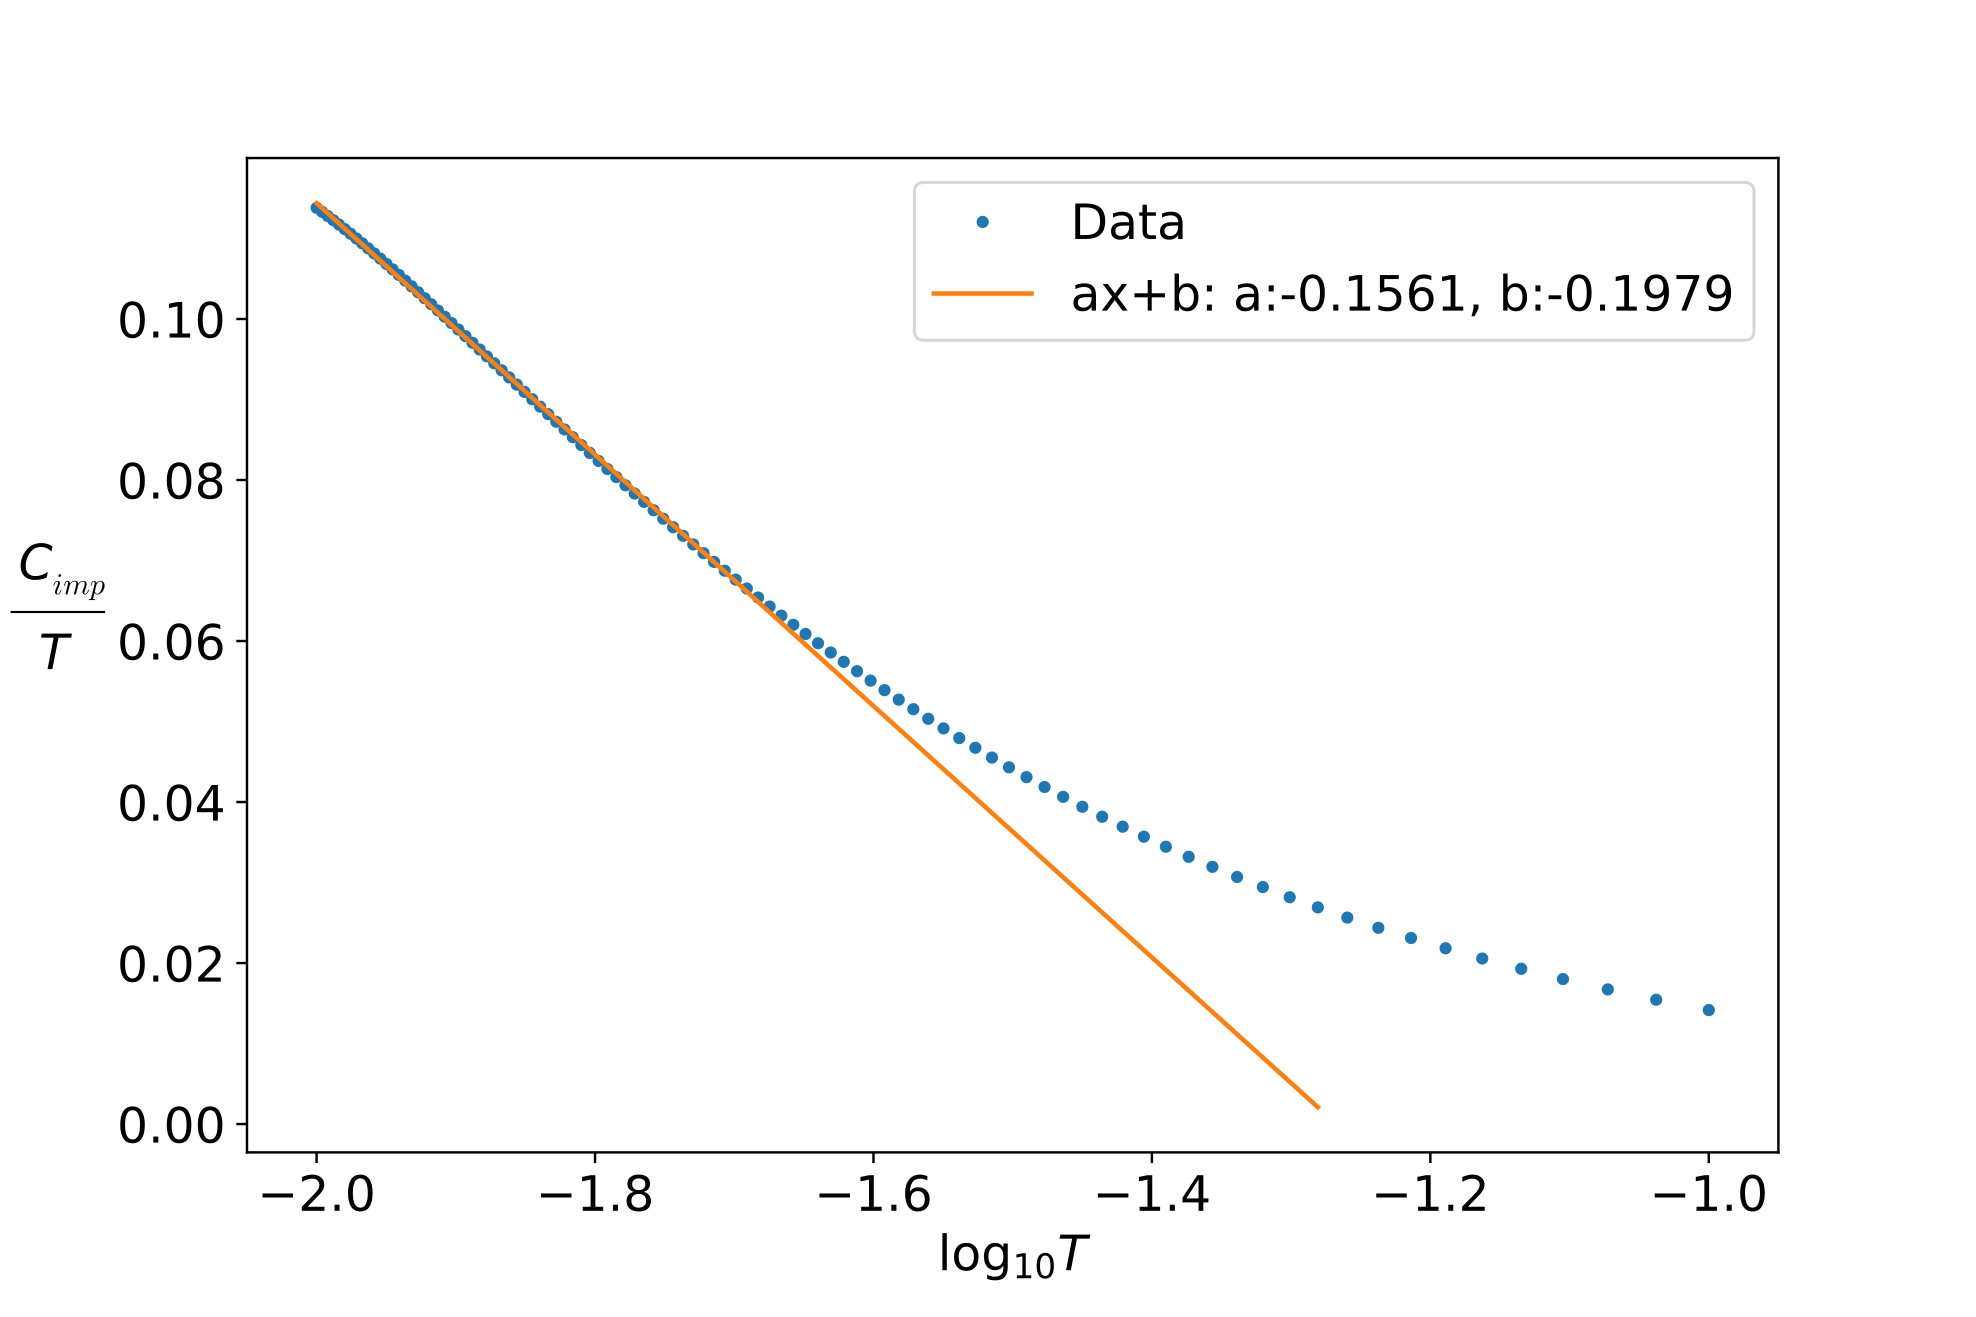
\includegraphics[scale=0.36]{plt/FINAL_fitted_Cv_t_0p1.png}
\caption{This figure shows the variation of the impurity specific heat with the temperature.}
\label{fig:Cv_imp}
\end{figure}
The above Fig.\ref{fig:Cv_imp} shows that at low temperature follows logarithmic behavior for the single channel case which is in agreement with the results known in the literature [CITE].
\begin{eqnarray}
\frac{C_{imp}}{T} \propto \log T
\end{eqnarray}


\subsubsection{Exact diagonalization}
Here we do the exact diagonalization the NFL Hamiltonian eq.\eqref{eq:hamiltonian_NFL} and find the eigenspectrum. Using this eigen spectrum  we computer various quantitites like $\chi$. We can compute other quantities from this exact diagonalization. 
\begin{eqnarray}
\chi &=& \beta\bigg[\frac{\sum e^{-\beta \bar{\epsilon}_{\Lambda}} \langle \bar{S}^{z2} \rangle}{\sum e^{-\beta \bar{\epsilon}_{\Lambda}} } -\frac{\sum e^{-\beta \epsilon_{\Lambda}} \langle S^{z2 }\rangle }{\sum e^{-\beta \epsilon_{\Lambda}} } \bigg] 
\end{eqnarray}
We numerically compute the $\chi$ from the definition above and study it's dependence on temperature.
\begin{figure}[!h]
\centering
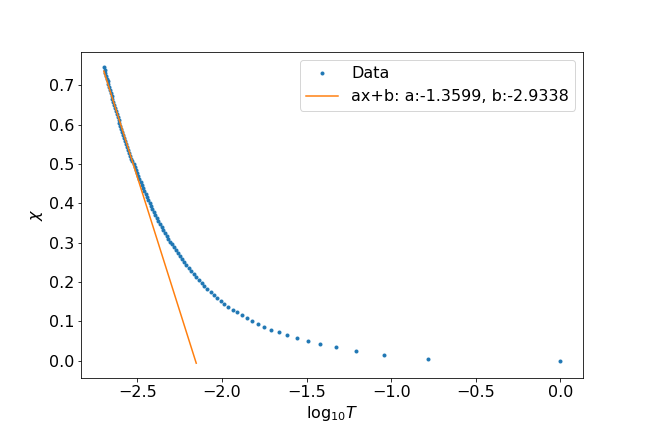
\includegraphics[scale=0.36]{plt/NFL_Chi_log_0p1}
\end{figure}
The above figure shows that at low temperture
\begin{eqnarray}
\chi(T) &\propto& \log T
\end{eqnarray}
This matches with the already known result of the literature. The ratio $\frac{\chi(T)}{C_{imp}/T} \sim 8.3$ greater than the Wilson ration. One can check this quantity for larger system size and at lower temperature for an better agreement.


\subsubsection{Momentum space structure of the NFL}
Direct fourier transformation on the $H^{(2)}_{off}$ leads to the LEH in momentum space showing higher order scattering involving electronic degree of freedoms.
%\begin{eqnarray}
%H_{eff}^{off,(2)} \bigg|_{diag} &=&  \frac{4t^2}{3\alpha} \bigg[ \frac{1}{N} \displaystyle\sum_{k,\sigma} n_{k\sigma}-\frac{1}{N^2} \displaystyle\sum_{k_1,k_2,\sigma} n_{k_1,\sigma} n_{k_2,-\sigma} \bigg] \times \bigg[\frac{1}{N} \displaystyle\sum_{k_1,\sigma} \tilde{n}_{k_1,\sigma} -  \frac{1}{N^2} \displaystyle\sum_{k_1,k_2,\sigma} \tilde{n}_{k_1\sigma}\tilde{n}_{k_2,-\sigma}\bigg] \nonumber\\
%\end{eqnarray}
The Fourier transformation of the electronic creation operator gives
%\begin{eqnarray}
%c_{r\sigma}^{\dagger} &=& \frac{1}{\sqrt{N}} \displaystyle\sum_{k} e^{-ikr} c_{k\sigma}^{\dagger}~,~\rightarrow c_{r\sigma} = \frac{1}{\sqrt{N}} \displaystyle\sum_{k} e^{ikr} c_{k\sigma} \nonumber\\
%c_{r,\sigma}^{\dagger} c_{r,-\sigma} &=& \frac{1}{N} \displaystyle\sum_{k,k'} e^{-i(k-k')r} c_{k,\sigma}^{\dagger} c_{k',-\sigma}    \nonumber\\
%n_{r\sigma}&=& c_{r\sigma}^{\dagger}c_{r\sigma} = \frac{1}{N} \displaystyle\sum_{k,k'} e^{-i(k-k')r} c_{k\sigma}^{\dagger} c_{k'\sigma} \nonumber\\
%n_{r\uparrow}n_{r\downarrow} &=& \frac{1}{N^2} \displaystyle\sum_{\substack{k_1,k_2\\k_3,k_4}} e^{-i(k_1-k_2)r} e^{-i(k_3-k_4)r} c_{k_1\uparrow}^{\dagger} c_{k_2\uparrow} c_{k_3\downarrow}^{\dagger} c_{k_4\downarrow}  
%\end{eqnarray}
%
%\begin{eqnarray}
%n_{r\uparrow}+n_{r\downarrow}-2n_{r\uparrow}n_{r\downarrow} &=& \frac{1}{N} \displaystyle\sum_{k,k',\sigma} e^{-i(k-k')r} c_{k\sigma}^{\dagger} c_{k'\sigma} -\frac{2}{N^2} \displaystyle\sum_{\substack{k_1,k_2\\k_3,k_4}} e^{-i(k_1-k_2)r} e^{-i(k_3-k_4)r} c_{k_1\uparrow}^{\dagger} c_{k_2\uparrow} c_{k_3\downarrow}^{\dagger} c_{k_4\downarrow}   \nonumber\\
%\textrm{The diagonal piece from this}  &\Downarrow & \nonumber\\
%&& \frac{1}{N} \displaystyle\sum_{k,\sigma} n_{k\sigma}-\frac{2}{N^2} \displaystyle\sum_{k_1,k_2} n_{k_1\uparrow} n_{k_2\downarrow}
%\end{eqnarray}


Thus one gets,
\begin{eqnarray}
(S_1^z)^2 \bigg|_{diag} &=& \frac{1}{4} (n_{1\uparrow}-n_{1\downarrow})^2\bigg|_{diag}=(n_{1\uparrow}+n_{1\downarrow}-2n_{1\uparrow}n_{1\downarrow})/4 \bigg|_{diag}\nonumber\\
%&=& \frac{1}{4N} \displaystyle\sum_{k,\sigma} n_{k\sigma}-\frac{1}{2N^2} \displaystyle\sum_{k_1,k_2} n_{k_1\uparrow} n_{k_2\downarrow} \nonumber\\
&=& \frac{1}{4N} \displaystyle\sum_{k,\sigma} n_{k\sigma}-\frac{1}{4N^2} \displaystyle\sum_{k_1,k_2,\sigma} n_{k_1,\sigma} n_{k_2,-\sigma}
\end{eqnarray}
We know that the diagoanl peice of the following terms is given as
%\begin{eqnarray}
%c_{r,\uparrow}^{\dagger} c_{r,\downarrow}  c_{r',\uparrow} c^{\dagger}_{r',\downarrow} &=& \frac{1}{N^2} \displaystyle\sum_{\substack{k_1,k_2\\k_3,k_4}} e^{-i(k_1-k_2)r} e^{-i(k_3-k_4)r} c_{k_1,\uparrow}^{\dagger} c_{k_2,\downarrow} c_{k_4,\uparrow}c_{k_3,\downarrow}^{\dagger}  \bigg|_{diag} \nonumber\\
%%&\Downarrow & \nonumber\\
%%&& \frac{1}{N^2} \displaystyle\sum_{\substack{k_1,k_2}} e^{-i(k_1-k_2)r} e^{-i(k_2-k_1)r} c_{k_1,\uparrow}^{\dagger} c_{k_2,\downarrow} c_{k_1,\uparrow}c_{k_2,\downarrow}^{\dagger}  \bigg|_{diag} \nonumber\\
%&=& -\frac{1}{N^2} \displaystyle\sum_{k_1,k_2} n_{k_1\uparrow}(1-n_{k_2\downarrow})
%\end{eqnarray}

Thus the diagonal piece coming from the term,
\begin{eqnarray}
&& c_{2\uparrow}^{\dagger}c_{2\downarrow} \bigg(  c_{l_1\uparrow}c_{l_1\downarrow}^{\dagger} +  c_{l_2\uparrow}c_{l_2\downarrow}^{\dagger} \bigg)\Rightarrow \frac{1}{N} \displaystyle\sum_{k,k'} e^{-i(k-k')r} c_{k,\sigma}^{\dagger} c_{k',-\sigma}  \nonumber
\end{eqnarray}
\begin{widetext}
Thus we get the diagonal correction of effective Hamiltonian in the momoentum spcae,
\begin{eqnarray}
H_{eff}^{off,(2)} \bigg|_{diag} &=& -\frac{8t^2}{3} \bigg[ \frac{1}{4N} \displaystyle\sum_{k,\sigma} n_{k\sigma}-\frac{1}{2N^2} \displaystyle\sum_{k_1,k_2} n_{k_1\uparrow} n_{k_2\downarrow} \bigg] \times \bigg[\frac{1}{N^2} \displaystyle\sum_{k_1,k_2} \tilde{n}_{k_1\uparrow}(1-\tilde{n}_{k_2\downarrow}) + (\uparrow \rightarrow \downarrow)\bigg] \times 2 \nonumber\\
%&=& -\frac{2t^2}{3} \bigg[ \frac{1}{N} \displaystyle\sum_{k,\sigma} n_{k\sigma}-\frac{2}{N^2} \displaystyle\sum_{k_1,k_2} n_{k_1\uparrow} n_{k_2\downarrow} \bigg] \times \bigg[\frac{1}{N} \displaystyle\sum_{k_1,\sigma} \tilde{n}_{k_1,\sigma} -  \frac{1}{N^2} \displaystyle\sum_{k_1,k_2,\sigma} \tilde{n}_{k_1\sigma}\tilde{n}_{k_2,-\sigma}\bigg]\times 2 \nonumber\\
&=& -\frac{4t^2}{3} \bigg[ \frac{1}{N} \displaystyle\sum_{k,\sigma} n_{k\sigma}-\frac{1}{N^2} \displaystyle\sum_{k_1,k_2,\sigma} n_{k_1,\sigma} n_{k_2,-\sigma} \bigg] \times \bigg[\frac{1}{N} \displaystyle\sum_{k_1,\sigma} \tilde{n}_{k_1,\sigma} -  \frac{1}{N^2} \displaystyle\sum_{k_1,k_2,\sigma} \tilde{n}_{k_1\sigma}\tilde{n}_{k_2,-\sigma}\bigg]~,~~~~ 
\end{eqnarray}
%
%
%\begin{eqnarray}
%H_{eff}^{off,(2)} \bigg|_{diag} &=&  -\frac{4t^2}{3} \bigg[ \frac{1}{N} \displaystyle\sum_{k,\sigma} n_{k\sigma}-\frac{1}{N^2} \displaystyle\sum_{k_1,k_2} n_{k_1,\sigma} n_{k_2,-\sigma} \bigg] \times \bigg[\frac{1}{N} \displaystyle\sum_{k_1,\sigma} \tilde{n}_{k_1,\sigma} -  \frac{1}{N^2} \displaystyle\sum_{k_1,k_2,\sigma} \tilde{n}_{k_1\sigma}\tilde{n}_{k_2,-\sigma}\bigg] \nonumber\\
%\label{eq:off-ham-110}
%\end{eqnarray}


\end{widetext}

\noindent Where $n_{k,\sigma}$ and $\tilde{n}_{k,\sigma}$ are the occupation of the states $k,\sigma$ corresponding to two different channels. One can define the charge density of $i^{th}$ channel with the spin-$\sigma$ as 
\begin{eqnarray}
q_{i,\sigma}=\frac{Q_{i,\sigma}}{N}=\frac{1}{N}  \displaystyle\sum_{k} n_{k,\sigma}
\end{eqnarray}
Thus one can re-write the abeove equation as,
\begin{eqnarray}
H_{eff}^{off,(2)} \bigg|_{diag} &=& -\frac{4t^2}{3} \prod_{i=\{1,2\}} \bigg[q_{i,\uparrow}+q_{i,\downarrow}-q_{i,\uparrow}q_{i,\downarrow}\bigg] \nonumber\\
\end{eqnarray}
This shows the inter-channel charge coupling present in the excitation spectrum.


\subsection{Third order}


\noindent Thus the off-diagonal part of the effective low energy Hamiltonian in the 2nd order is
\begin{eqnarray}
&&H_{eff, off}^{(2)} 
= \frac{J^2}{\alpha}\bigg[ c_{1\uparrow}c_{1\downarrow}^{\dagger} \bigg(-\alpha\beta \bigg\{\Sigma_{3,2} + c_{3\uparrow}^{\dagger} c_{3\downarrow} c_{2\uparrow} c_{2\downarrow}^{\dagger} \bigg\}-\alpha\gamma \Omega_{3,2}\bigg) \nonumber\\
&&~~~~+c_{2\uparrow}c_{2\downarrow}^{\dagger} \bigg(-\alpha\beta \bigg\{\Sigma_{1,3} + c_{1\uparrow}^{\dagger} c_{1\downarrow} c_{3\uparrow} c_{3\downarrow}^{\dagger} \bigg\}-\alpha\gamma \Omega_{1,3}\bigg) \nonumber\\
&&~~+c_{3\uparrow}c_{3\downarrow}^{\dagger} \bigg(-\alpha\beta \bigg\{\Sigma_{2,1} + c_{2\uparrow}^{\dagger} c_{2\downarrow} c_{1\uparrow} c_{1\downarrow}^{\dagger} \bigg\}-\alpha\gamma \Omega_{2,1}\bigg) + \textrm{h.c.} \bigg]
\nonumber\\
&&~~~~~~~~~~~~~~~\otimes \bigg[ c_{l_1\uparrow}^{\dagger} c_{l_1\downarrow} +c_{l_2\uparrow}^{\dagger} c_{l_2\downarrow} + c_{l_3\uparrow}^{\dagger} c_{l_3\downarrow} + \textrm{h.c.}\bigg] \nonumber
\end{eqnarray} 
 \begin{eqnarray}
\Sigma_{i,j} &=&-8S_i^zS_j^z  [  (C^z_i-C^z_j  )^2  + (S_i^z-S_j^z  )^2  ] \\
\Omega_{i,j} &=& 4S_i^z S_j^z (C_i^z+C_i^z)(C_j^z+C_j^z)
\end{eqnarray}

 
\noindent Now we are interested calculating the diagonal part of the effective Hamiltonian. In this case we get non-zero contribution from all the three ground states $|J^z=-1\rangle$, $|J^z=0\rangle$ and $|J^z=1\rangle$.
We get the diagonal contribution to the LEH in the second order is 
\begin{eqnarray}
H^{(2)}_{eff, diag} &=& - \frac{7.2 J^2}{\alpha} \hat{I}
\end{eqnarray}
The contribution associater to different ground states $|J^z=-1\rangle$, $|J^z=0\rangle$ and $|J^z=1\rangle$ is given respectively as $- \frac{2.4 J^2}{\alpha} \hat{I} + \hat{\mathcal{F}},- \frac{2.4 J^2}{\alpha} \hat{I} ,- \frac{2.4 J^2}{\alpha} \hat{I} - \hat{\mathcal{F} }$,
\noindent where $\hat{\mathcal{F}}$ is a function of diagonal number oprators of the nearest-neighbor site degree of freedom $l_1,l_2,l_3$ etc.




\section{Channel Anisotropy and Berry phase}

noindent Here we start with the multi-channel zero mode model, any put anisotropy in the counping $\alpha$. Let's start with a simpe possibility where there are two coupling $\alpha_1$ and $\alpha_2$, where both the $\alpha_1,\alpha_2$ are positive and negative. We write down the Hamiltonian corresponding to these cases,
\begin{eqnarray}
H_{an}&=& \alpha_1 \vec{S}_d.\vec{S}_1 + \alpha_2 \vec{S}_d.\vec{S}_2 %\\
%&=& \frac{\alpha_1}{2} (J_1^2-S_d^2-S_1^2) + \frac{\alpha_2}{2} (J_2^2-S_d^2-S_2^2)
\end{eqnarray}
%Now let's find out the CSCO for this above Hamiltonian. The operators which commutes with the Hamiltonian are $J_1,J_2,S_d,S_1,S_2$. Now can we choose the basis to be, 
%\begin{eqnarray}
%|J_1^z,S_1^z\rangle \otimes |S_d^z\rangle \otimes |J_2^z,S_2^z\rangle
%\end{eqnarray}
%In the ground state both the $S_1$ and $S_2$ will be maximum and $J_1$ and $J_2$ will be minimum. 
%\begin{enumerate}
%\item Term 1: $S_1=N_1/2$, where $N_1$ is the number of outer spin connected with the central spin with the coupling constant $J_1$. There are two possible $J_1$ values $J_1=(S_1+1/2)$ and $J_1=(S_1-1/2)$. In the ground state the being maximum $J_1=(S_1-1/2)$. Thus the energy contribution to the ground state from the the first term is 
%\begin{eqnarray}
%-\frac{\alpha_1(S_1+1)}{2}
%\end{eqnarray}
%
%\item Term 2: Similar calculation show the contribution of the second term in the ground state energy is
%\begin{equation}
%-\frac{\alpha_2(S_2+1)}{2}
%\end{equation}
%Thus total ground state energy is 
%\begin{eqnarray}
%E_g  &=& -\frac{\alpha_1(S_1+1)}{2}-\frac{\alpha_2(S_2+1)}{2}
%\end{eqnarray}
%
%\end{enumerate}
%
%
%%In this ground state there are $2S_1$ number of $J_1^z$ eigen values with same energy contribution and similarly there are $2S_2$ number of $J_2^z$ states with same energy. Thus we can write down the ground state as 
%%\begin{eqnarray}
%%&& |J_1^z,S_1^z\rangle \otimes |S_d^z\rangle \otimes |J_2^z,S_2^z\rangle \nonumber\\
%%&=& |J_1,J_1^z\rangle \otimes |J_2,J_2^z\rangle
%%\end{eqnarray}
%
%
%One cna solve this problem in another way by rewriting the Hamiltonian as
%\begin{eqnarray}
%H=
%\end{eqnarray}
%
There are $K_1$ and $K_2$ numbers of outer spins respectivelty which are connected to the central spin with the coupling with $\alpha_1$ and $\alpha_2$. Thus the total number of channels is $K=K_1+K_2$. When $\alpha_1=0, \alpha_2\neq 0$ then we end up with a multi-channel problem with $K_1$ number of channels thus the degeneracy becomes $K_1$ and for $\alpha_2=0, \alpha_1\neq 0$ the degneracy becomes $K_2$. Though this can be trivially verified from the above Hamiltonian, the important property of this problem is the robustness of the ground state degeneracy. As we vary $\alpha_1$ and $\alpha_2$, to study the ground state degeneracy. We find that for any values $\alpha_1$  and $\alpha_2$ such that $\alpha_1/\alpha_2\neq 0$ and $\alpha_2/\alpha_1\neq 0$ the ground state degeneracy remains constant at $K=K_1+K_2$. It is known in the literature [CITE someone] that under above mentioned an-isotropy the low energy effective Hamiltonian becomes a multi-channel Kondo with smaller number of channels.

\begin{figure}\centering
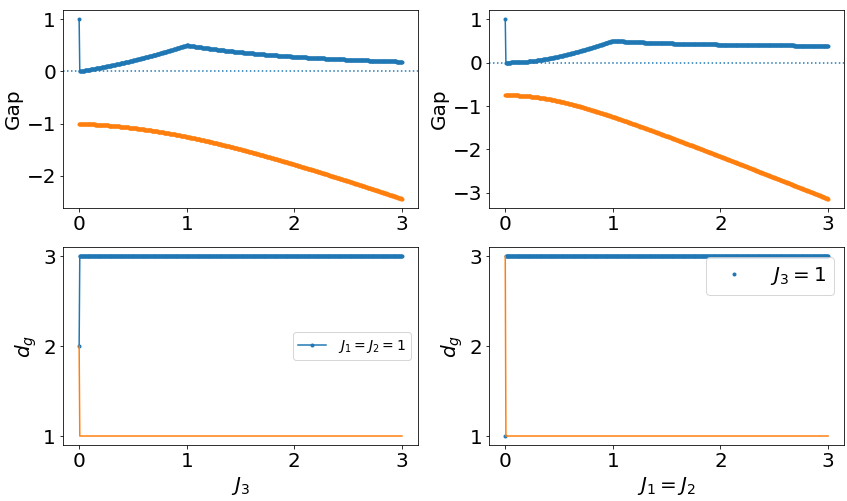
\includegraphics[width=0.5\textwidth]{plt/Anisotropy_Channel:3}
%{example-image-a}
\caption{Add proper figures.}
\end{figure}


\subsection{Berry phase}

We start with the general multi-channel problem where the coupling strength with the central impurity spin of the $i^{th}$ channel is $\alpha_i$. Here our goal is to use the robustness of the ground state degeneracy of the star-graph model to build the gaue theoretic structure. We define the hamiltonian of star-graph as 
\begin{eqnarray}
H_{st}(\vec{\alpha}) &=& \displaystyle\sum_{i=1}^{K} \alpha_i \vec{S}_d.\vec{S}_i
\end{eqnarray}
We define the $K$-dimensional soupling space where one possible sonfiguration is denoted by the vector $\vec{\alpha}=\mathcal{N}(\alpha_1,\alpha_2,\cdots,\alpha_K)$, where $\mathcal{N}$ is the normalization factor, where $\alpha_i\neq 0$ and $\alpha_i\neq \infty $, $\forall i\in[K]$. The Schrodinger equation for the Hamiltonian reads as 
\begin{eqnarray}
H_{st}(\vec{\alpha}) \Psi_{m} (\vec{\alpha}) = E_{m} (\vec{\alpha}) \Psi_{m} (\vec{\alpha})
\end{eqnarray}
Here, we are only interested in the ground state manifold, where the energy of the state is $E_{g}$. Due to the degeneracy ($K$-fold) there are $K$ states in that manifold with the same energy labeled by say $k$. Thus the equation for the ground state manifold reads
\begin{eqnarray}
H_{st}(\vec{\alpha}) \Psi^{k}_{g} (\vec{\alpha}) = E_{g} (\vec{\alpha}) \Psi^{k}_{g} (\vec{\alpha})
\end{eqnarray}
One can do a simple transformation to make the ground state energy zero. Thus
\begin{eqnarray}
H_{st}(\vec{\alpha}) \Psi^{k}_{g} (\vec{\alpha}) &=&  0 \nonumber\\
i\hbar \frac{\partial \Psi(\vec{\alpha(t)}) }{\partial t} &=& H_{st}(\vec{\alpha(t)}) \Psi(\vec{\alpha(t)}) =0
\label{eq:hamiltonian_eq}
\end{eqnarray}
As the ground state is degenerate one can take any linera combinations of the states to create arbitrary basis state (orthogonal and normalized). Let's say $\psi_k(\vec{\alpha}(t))$ represents the arbitrary basis state, which should  be smooth in $t$ locally and follow the Schrodinger equation,
\begin{eqnarray}
H_{st}(\vec{\alpha}(t)) \psi_k(\vec{\alpha}(t)) &=&  0 
\end{eqnarray}
We here try to find the solution of the Eq.\eqref{eq:hamiltonian_eq}, we start with the trial solution 
\begin{eqnarray}
\eta_a(t) &=& U_{ab}(t) \psi_b(t)
\end{eqnarray}

\textbf{Finish this section.}


 \section{Topology and Gauge theory}




%\subsection{Gauge theory and Wilson Loops}
%
%%\subsection{Twist-translation operator}
%\noindent We define a translation operator $\hat{T}$ and twist operator $\hat{O}$ to describe the ground state manifold. The ground state manifold has $K$ fold degeneracy, labeled by the eigenvalue of the translation operator. The hamiltonain H commutes with the translation operator $[H,\hat{T}]=0$. We define the twist and tranlation operators in terms of an exponential of another operators as shown below.
%
%\begin{eqnarray}
%\hat{T}&=& e^{i\hat{P}} ~,~~\hat{O}=e^{i\hat{Q}}
%\end{eqnarray}
%We label the K degenerate eigenstates as $|p_i\rangle$ where $i\in [K]$ and the action of the translation operator on those states are given as 
%\begin{eqnarray}
%\hat{T} |p_m\rangle &=& e^{ip_m}~,~\textrm{where $\hat{P} |p_m\rangle=p_m |p_m\rangle$}
%\end{eqnarray}
%Now we discuss the property of the twist operator. The twist operator takes one state $|p_m\rangle$ to the nearest state $|p_{m+1}\rangle$.
%\begin{eqnarray}
%\hat{O} |p_m\rangle &=& |p_{m+1}\rangle~. ~~\textrm{or very generally} \\
%\hat{O}^{n} |p_m\rangle &=& |p_{(m+n) \textrm{mod} K}\rangle~.
%\end{eqnarray}
%Thus the above two equation seeks the wilson loop relation as
%\begin{eqnarray}
%\hat{T}\hat{O}^{n} |p_{m}\rangle &=&  \hat{T} |p_{(m+n) \textrm{mod} K} \rangle = e^{i\gamma_{m,n}} |p_{(m+n) \textrm{mod} K} \rangle \\
%\hat{O}^{n} \hat{T} |p_{m}\rangle &=& \hat{O}^{n} e^{ip_m} |p_{m}\rangle = e^{ip_m} |p_{(m+n) \textrm{mod} K} \rangle 
%\end{eqnarray}
%where $\gamma_{m,n}=p_{(m+n) \textrm{mod} K}+ (K-m)$. Thus we get the phase difference
%\begin{eqnarray}
%\langle p_{m} | \hat{T}^{\dagger} \hat{O}^{n \dagger} \hat{T}\hat{O}^{n} |p_{m}\rangle &=& e^{i[\gamma_{m,n}-p_{m}]} \equiv e^{i\frac{2n\pi}{K}}
%\end{eqnarray}
%
%
%Another way of finding out the structure of $\hat{O}$ is to use the BCH expansion. We know that for a two genral oeprators $X,Y$ we get 
%\begin{eqnarray}
%e^{X}Ye^{-X} &=& Y+[X,Y]+\frac{1}{2!}[X,[X,Y]]+\frac{1}{3!}[X,[X,[X,Y]]]+ \cdots.
%\end{eqnarray}
%Using the above formula we can calculate
%\begin{eqnarray}
%\hat{T}\hat{O}^{n}\hat{T}^{\dagger} &=& e^{i\hat{P}} \hat{O}^{n} e^{-i\hat{P}} = \hat{O}^{n} e^{in\theta} \nonumber\\
%&=& \hat{O}^n + [i\hat{P},\hat{O}^n] + \frac{1}{2!} [i\hat{P},[i\hat{P},\hat{O}^n]] + \frac{1}{3!} [i\hat{P}, [i\hat{P},[i\hat{P},\hat{O}^n]]] + \cdots  \nonumber\\
%&=& \hat{O}^{n} \bigg[ 1+ (in\theta) + \frac{(in\theta)^2}{2!} + \frac{(in\theta)^3}{3!} + \cdots \bigg]
%\end{eqnarray}
%Assummption from the above equation is 
%\begin{eqnarray}
%[i\hat{P},\hat{O}^n] &=& i(n\theta) \hat{O}^{n} ~,~\textrm{which leads to }
%\end{eqnarray}
%\begin{eqnarray}
%[i\hat{P},[i\hat{P},\hat{O}^n]] &=&  [i\hat{P},\hat{O}^{n}] i(n\theta)  =\hat{O}^n (in\theta)^2
%\end{eqnarray}
%and so on. Thus the assumption is correct. Thus we get the commutation relation
%\begin{eqnarray}
%[ \hat{P},\hat{O}^n] &=& ( n\theta) \hat{O}^n 
%\end{eqnarray}
%\begin{eqnarray}
%[\hat{P},e^{in\hat{Q}}] &=& (n\theta) e^{in\hat{Q}}~,~\textrm{$\forall n$.}
%\end{eqnarray}
%%This implies,
%%\begin{eqnarray}
%%[\hat{P},e^{in\hat{Q}}] &=& [\hat{P},1+(in\hat{Q})+\frac{(in\hat{Q})^2}{2!}+\frac{(in\hat{Q})^3}{3!} +\cdots]  \nonumber\\
%%&=& [\hat{P},1]+  [\hat{P},(in\hat{Q})]+  [\hat{P},\frac{(in\hat{Q})^2}{2!}]+  [\hat{P},\frac{(in\hat{Q})^3}{3!} +\cdots] \nonumber\\
%%&=& (n\theta) \bigg[ 1+ (in\hat{Q}) + \frac{(in\hat{Q})^2}{2!} +\frac{(in\hat{Q})^3}{3!} +\cdots \bigg]
%%\end{eqnarray}
%%Above equation leads to a trial solustion 
%%\begin{eqnarray}
%%[\hat{P},(in\hat{Q})^r]=(n\theta) (in\hat{Q})^r~,~r=0,1,2,\cdots
%%\end{eqnarray}
%
%
%\noindent We are intrested in the simple case where $[\hat{P},\hat{Q}]=\hat{\Gamma} \neq 0$ and $[\hat{\Gamma},\hat{P}]=0=[\hat{\Gamma},\hat{Q}]$. In this case we get 
%\begin{eqnarray}
%e^{i\hat{P}} e^{i\hat{Q}} e^{-i\hat{P}} &=& e^{i\hat{Q}} e^{-[\hat{P},\hat{Q}]}
%\end{eqnarray}

%
%\subsection{LSM style calculation}
%
%\noindent In standard LSM style study and in it's various generalizations we usually define two operators, translation $\hat{T}$ and twist operator $\hat{O}$. We take the system and add a periodic boundary condition along one direction, let's say $\hat{x}$. Then we insert the gauge flux through that closed loop formed by the periodic $x-$direction. Let's for example take a spin problem shere each point along the $x-$axis there is a spin-1/2 object sitting. The Hamiltonian of that spin problem is $H_{lsm}$. By construction, this Hamiltonian has the translation symmetry along the $x-$direction. Thus this hamiltonian commutes with the translation operator along the $x-$direction denoted as $\hat{T}_x$, and the commutation reads $[\hat{T}_x,\hat{H}_{lsm}]=0$. Now we define the twist operator $\hat{O}$ as 
%\begin{eqnarray}
%\hat{O} &=& e^{i\frac{2\pi}{N_x} \displaystyle\sum_{\vec{r}} x S_{\vec{r}}^z }~.~
%\end{eqnarray}
%This twist operator inserts one full $2\pi$ flux into the system. In genral this full twist operator does not commutes with the Hamiltonian, we first study the commutation ralation.
%\begin{eqnarray}
%[\hat{H}_{lsm},\hat{O}] &\neq & 0
%\end{eqnarray}
%This commutation relation totally depends on the microscopic structure of the Hamiltonian $H_{slm}$. We can though study the commutation relation between this twist operator and the translation operator. This does not needs the microscopic knowledge of the Hamiltonian. This is assuming the fact that the spins are equally spaced along the $x-$direction and $xS^z_{\vec{r}}\equiv x\sum_{y} S^z_{(x,y)}$, where $\vec{r}=(x,y)$. In the general cases where the arrangement of the spin along the $x-$direction is non-trivial function of the $x-$coordinate, we can write the twist operator as 
%\begin{eqnarray}
%\hat{O} &=& e^{i\frac{2\pi}{N_x} \displaystyle\sum_{\vec{r}, x=1}^{N_x} f_x S_{\vec{r}}^z }~.~
%\end{eqnarray}
%Whatever be the general structure there should be translation invariance in the problem. The the brading rules between the twist and the translation operators for the simle case of problems where the spacings are uniform/trivial are given as 
%\begin{eqnarray}
%\hat{T} \hat{O} \hat{T}^{\dagger} &=&  \hat{O}  \times e^{-\frac{2\pi}{N_x} S^z_{tot}} \times  e^{i 2\pi \sum_{y} S^z_{1,x}}
%\end{eqnarray}
%Sofar the calculations are in the operetor level, now we invoke the ground state property. We take the ground state value of the total magnetizaion $S^z_{tot}$. For the special case, where in the ground state $S^z_{tot}=0$, we get
%\begin{eqnarray}
%\hat{T} \hat{O} \hat{T}^{\dagger} &=&  \hat{O}    \times  e^{i 2\pi \sum_{y} S^z_{1,x}}
%\end{eqnarray}
%Now based on the value of $\sum_{y} S^z_{1,x}$ integer/half-integer we get trivial/non-trivial braiding rules between the twist and translation operators. We are interested in the non-trivial case here, which yields
%\begin{eqnarray}
%\hat{T} \hat{O} \hat{T}^{\dagger} &=&  \hat{O}    e^{\pm i\pi}
%\label{eq:TOTpOp_pi}
%\end{eqnarray}
%Now, let's assume that $|\psi_0\rangle$ is the ground state of the problem. Sofar, we have no idea about the nature of the gruond state and the excited states. As the translation operator is commuting, then the generator of this translation opertion $\hat{P}$ ($\hat{T}=e^{i\hat{P}}$) will also commute with the Hamiltonian.  Thus we can label the states with the eigenvalules of this operator $\hat{P}$.
%\begin{eqnarray}
%\hat{T} |p_1\rangle &=& e^{ip_1} |p_1\rangle~,~
%\end{eqnarray}
%Now from the eq.\eqref{eq:TOTpOp_pi} we can check the action of the operator $\hat{O}$ on the ground state $|p_1\rangle \equiv |\psi_0\rangle$. We find that
%\begin{equation}
%\langle p_1| \hat{O}|p_1\rangle =0
%\end{equation}
%Thus $|p_1^{(1)}\rangle \equiv \hat{O} |p_1\rangle$ is orthogonal to the ground state $|p_1\rangle$. Now we need to find out the energy difference between $|p_1\rangle$ and $|p_1^{(1)}\rangle$. To calculate that we need to find out the expectation value
%\begin{eqnarray}
%\Delta E &=&  \langle p_1^{(1)}| \hat{H}_{lsm}|p_1^{(1)}\rangle - \langle p_1| \hat{H}_{lsm}|p_1\rangle  \nonumber\\
%  &=&  \langle p_1 | \hat{O} \hat{H}_{lsm} \hat{O}^{\dagger} |p_1\rangle - \langle p_1| \hat{H}_{lsm}|p_1\rangle 
%\end{eqnarray}
%\noindent In the case where the twist operator commutes with the Hamiltonian $[\hat{H}_{lsm},\hat{O}]=0$, we will get $\Delta E=0$ in the operator level, independent of the system size. For the case $\Delta E=0$ we can say that ground state is doubly degenerate, labeled by the two eigen values of the momentum operator $0$ and $\pi$.
%
%\par But in the LSM case this twist operator does not commute with the Hamiltonian, thus in general $\Delta E\neq 0$. For this case we can see that the twisted state is an excited state. In special problem it can be shown that in the termodynamic limit this gap $\Delta E$ vanishes, showing either the double degenerate ground state (if one can show a gap above) or gapless spectrum.
%
%\subsubsection{Special case in fractional QHE}
%\noindent In the quantum hall problem, we can write down the Hamiltonian as 
%\begin{eqnarray}
%H_{qh} &=& \frac{1}{2m} \bigg[ \Pi_x^2 + \Pi_y^2\bigg]~,~  \textrm{where}~~ \vec{\Pi}=-i\hbar \vec{\nabla} + e\vec{A}
%\end{eqnarray}
%We know $[\Pi_x,\Pi_y]\neq 0$ thus the Hamiltonian also does not commutes with these operators individually. But one can define a pseudo-momentum $\tilde{\Pi}_{x/y}$ which commutes with the Hamiltonian in a particular gauge choice. For an example in Tao \& Haldane 1985, landau gauge was chosen $\vec{A}=(0,Bx,0)$. In this Landau gauge thepseudo momentum defined was ${\tilde{\Pi}}_x=p_x+eBy$ and ${\tilde{\Pi}}_y=p_y$. This pseudo-momentum operators commutes with the Hamiltonian and does not commutes with each other thus, following the algebra of $\hat{P}$ and $\hat{Q}$ as described in the above section. One can easily check that $[\tilde{\Pi}_x,\tilde{\Pi}_y]=i\hbar eB$.\\
%
%
%\par \textit{Question:} Now the question is, for a general Hamiltonian $H_{gen}$, if the ground state is multiply degeenrate (morethan one mutually orthogonal states with same minimum energy available). Can we always find out two operators $\hat{P},\hat{Q}$ such that $[\hat{H},\hat{P}]=[\hat{H},\hat{Q}]=0$ and $[\hat{P},\hat{Q}]\neq i\hbar c$, where $c$ is a constant.

\subsection{In our case of stargraph model}
\noindent In our model we find two string operators $\hat{\mathbb{Z}}=\sigma_d^z\Pi_{i=1}^{K} \sigma_i^z$ and $\hat{\mathbb{X}}=\sigma_d^x\Pi_{i=1}^{K} \sigma_i^x$, where $K$ is the number of channels. These two operators commutes with the Hamiltonian $H$ of this stargraph.
\begin{eqnarray}
[H,\hat{\mathbb{Z}}] &=& 0 = [H,\hat{\mathbb{X}}]
\end{eqnarray}

We can rewrite the operators in the form of a twist operator as,
\begin{eqnarray}
\mathbb{Z} &=& \sigma_d^z\displaystyle\prod_{i=1}^{K} \sigma_i^z = \frac{1}{i^{K+1}} e^{i\frac{\pi}{2} \sum_{i} \sigma^z_i}=e^{i\frac{\pi}{2} \sum_{i} (\sigma^z_i -1) } =e^{i\pi \sum_{i} (S^z_i -1/2) }
\end{eqnarray}
Similarly one can rewrite
\begin{eqnarray}
\mathbb{X} &=& \sigma_d^x\displaystyle\prod_{i=1}^{K} \sigma_i^x =e^{i\pi \sum_{i} (S^x_i -1/2) }
\end{eqnarray}
The commutation between these two operators are given as
\begin{eqnarray}
[\mathbb{Z},\mathbb{X}] &=& \prod_{i=d,1}^{K} \sigma^z_{i} \prod_{i=d,1}^{K} \sigma^x_{i} \bigg[1-(-1)^{K+1}\bigg]
\end{eqnarray}
Thus we can see that for case where number of channels is odd that means $K+1$ is even, these two string operators commutes with each other forming a CSCO ($H,\hat{\mathbb{Z}},\hat{\mathbb{X}}$). On the other hand in the case where number of channels $K$ is even, these two operators does not commute with each other. Let's discuss these two cases seperately.
\subsubsection{$K=odd$} 
In the case where the number of channels $K$ is odd, we get $[\mathbb{Z},\mathbb{X}]=0$. Thus forming a CSCO with elements $H,\hat{\mathbb{Z}},\hat{\mathbb{X}}$. Thus one can label the states using the eigenvalues of these operators. For the case of $K=2n+1$ channels, the grounf state is $K$ fold degenerate and labeled by the eigenvalues of the operator $J^z$ which can take values $J^z=[-J,-J+1,\cdots, J-1, J]$, where $J=(K-1)/2$. For the odd channel case $J^z$ can take zero value. Thus 
\begin{eqnarray}
|J^z\rangle \equiv |Z,X \rangle
\end{eqnarray}
where the eigenvalue $Z$ can take $(K+1)/2$ values related to the absolute $|J^z|$ but cannot distinguish between $\pm J^z$ and $X$ can take two values $\pm 1$ which breaks the degenercy between $\pm J^z$. Thus these two operators together can uniquely label all the degenerate states.
% Note, the states $|Z=\rangle$

\subsection{Main}

\par We can define two operators, for convenience let's call translation and twist operator respectively, $\hat{T}$ and $\hat{O}$ defined as 
\begin{eqnarray}
\hat{T} &=& e^{i\frac{2\pi}{K} \hat{\Sigma}} ~,~\hat{O} = e^{i\hat{\phi}}~,~~\hat{\Sigma}=[\hat{J}^z-(K-1)/2]
\end{eqnarray}
One can see that the generators of these above operators commutes with the Hamiltoninan, $[H,J^x]=[H,J^z]=[H,J^z]=0$. In the large channel limit we can do semiclaassical approximation. As $J^x$ and $J^y$ both commutes with the Hamiltonian $H$ then $[H,J^y{(J^{x})}^{-1}]=0$, and any non-singular function of these operators must also commute with the Hamiltonian, thus we can say that
\begin{eqnarray}
\hat{\phi}=\tan^{-1}(\hat{J}^y(\hat{J}^x)^{-1})
\end{eqnarray}
Then we get $[\hat{\phi},\hat{H}]=0$. We can label the ground states by the eigen values of the translation operator $\hat{T}$. We can also use the ground states labeled by the eigenvalues of $J^z$ ($M$, say). Then the ground states are 
\begin{eqnarray}
|M_1\rangle,|M_2\rangle,|M_2\rangle,\cdots ,|M_K\rangle
\end{eqnarray}
Then the operations of the translation operators on this states are give below.
\begin{eqnarray}
\hat{T}|M_i\rangle &=& e^{i\frac{2\pi}{K} [M_i-(K-1)/2]} |M_i\rangle = e^{i2\pi\frac{p_i}{K} } |M_i\rangle~,~p_i\in[1,\cdots,K]
\end{eqnarray}
Now we check the braiding rule between the twist and the translation operators, we find
\begin{eqnarray}
\hat{T}\hat{O}\hat{T}^{\dagger}\hat{O}^{\dagger} &=& e^{\frac{2\pi }{K}[i\hat{\Sigma},i\hat{\phi}]}=e^{i\frac{2\pi }{K}} \nonumber\\
\hat{T}\hat{O}^m\hat{T}^{\dagger}\hat{O}^{\dagger m} &=& e^{\frac{2\pi }{K}[i\hat{\Sigma},im\hat{\phi}]}=e^{i2\pi \frac{m}{K}}
\end{eqnarray}

Next we shown that the states $\hat{O}^m |M_i\rangle$ are orthogonal to each other and with the state $|M_i\rangle$.

\begin{eqnarray}
\hat{T} \hat{O}^m |M_i\rangle &=& \hat{O}^m \hat{T} e^{i2\pi \frac{m}{K}} |M_i\rangle =\hat{O}^m e^{i \frac{2\pi(m+p_i)}{K} } |M_i\rangle \nonumber\\
\hat{T} \bigg(\hat{O}^m |M_i\rangle \bigg) &=&  e^{i \frac{2\pi(m+p_i)}{K} } \bigg( \hat{O}^m |M_i\rangle \bigg)
\end{eqnarray}
Thus different states $ \hat{O}^m |M_i\rangle$ for different $m$ are labeled by different eigenvalues of the translation operations, thus are orthogonal to each other. Now as the twist operator $\hat{O}$ commutes with the Hamiltonian, thus we can see that 
\begin{eqnarray}
\langle M_i| \hat{O}^{m \dagger}  H \hat{O}^m |M_i\rangle =\langle M_i|  H |M_i\rangle 
\end{eqnarray}
Thus the energy eigen values of all the orthogonal states are equal. Thus all the K mutually orthogonal states are degenerate.


\subsection{Fractional statistics}




\section{Local Mottliquid}


\noindent Using the unitary renormalization group method we decouple the impurity spin from the zero-modes of the $K$ channels. We start with the Hamiltonian. The zero mode Hamiltonian is a stargraph model 
\begin{eqnarray}
H &=& \alpha \vec{S}_d.\displaystyle\sum_i \vec{S}_i =\alpha S_d^zS^z + \frac{\alpha}{2} (S_d^+S^-+ S_d^-S^+) \nonumber\\
H_D &=& \alpha S^z_d S^z~,~~ H_X = \frac{\alpha}{2} (S_d^+S^-+ S_d^-S^+)
\end{eqnarray}
Here we want to remove the quantum fluctuations between the impurity spin and the rest, for that we do one step URG.

\begin{eqnarray}
\Delta H &=& H_X \frac{1}{\hat{\omega}-H_D} H_X \nonumber\\ 
%&=&\frac{\alpha^2}{4} \bigg[ S^- S_d^+ \frac{1}{\omega_{\uparrow}-\alpha S_d^zS^z} S^-_d  S^+  \bigg] +\frac{\alpha^2}{4} \bigg[ S^+ S_d^- \frac{1}{\omega_{\uparrow}-\alpha S_d^zS^z} S^+_d  S^-  \bigg] \nonumber\\
%&=&\frac{\alpha^2}{4} \bigg[ S^-S^+ S_d^+S^-_d \frac{1}{\omega_{\uparrow}-\alpha (S_d^z-1)(S^z+1)}     \bigg] +\frac{\alpha^2}{4} \bigg[ S^+S^- S_d^-S^+_d \frac{1}{\omega_{\downarrow}-\alpha (S_d^z+1)(S^z-1)}     \bigg] \nonumber\\
%&=&\frac{\alpha^2}{4} \bigg[ S^-S^+(1/2+S^z_d) \frac{1}{\omega_{\uparrow}-\alpha (S_d^z-1)(S^z+1)}     \bigg] +\frac{\alpha^2}{4} \bigg[ S^+S^-(1/2-S_d^z) \frac{1}{\omega_{\downarrow}-\alpha (S_d^z+1)(S^z-1)}     \bigg] \nonumber\\
\end{eqnarray}
In the zero mode IR fixed point ground state (stargraph) of multi-cahnnel ground state $J^z$ is a good quantum number but $S^z$ is not. There is no net $S^z$ field thus in the ground state manifold the average $S^z$ is vanishing, $\langle S^z \rangle=0$. We use this expectation value to replace the denominator of the above RG equation.

%\begin{eqnarray}
%\Delta H &=& \frac{\alpha^2}{4} \bigg[ S^-S^+ (1/2+S^z_d) \frac{1}{\omega_{\uparrow}-\alpha (S_d^z-1)(\langle S^z \rangle +1)}     \bigg] +\frac{\alpha^2}{4} \bigg[ S^+S^- (1/2-S_d^z) \frac{1}{\omega_{\downarrow}-\alpha (S_d^z+1)(\langle S^z \rangle-1)}     \bigg] \nonumber\\
%%&=& \frac{\alpha^2}{4} \bigg[ S^-S^+ (1/2+S^z_d) \frac{1}{\omega_{\uparrow}-\alpha (S_d^z-1 )}     \bigg] +\frac{\alpha^2}{4} \bigg[ S^+S^- (1/2-S_d^z) \frac{1}{\omega_{\downarrow}+\alpha (S_d^z+1) }     \bigg] \nonumber\\
%%&=& \frac{\alpha^2}{4} \bigg[ S^-S^+ (1/2+S^z_d) \Gamma_{\uparrow}\bigg] +\frac{\alpha^2}{4} \bigg[ S^+S^- (1/2-S_d^z) \Gamma_{\downarrow} \bigg] \nonumber\\
%&=& \frac{\alpha^2}{4} \bigg[ (S^2-S^{z2}- S^z)(1/2+S^z_d) \Gamma_{\uparrow} \bigg]+\frac{\alpha^2}{4} \bigg[ (S^2-S^{z2}+ S^z)(1/2-S^z_d) \Gamma_{\downarrow} \bigg] \nonumber\\
%\end{eqnarray}
%Due to unitary condition the $\omega_{\uparrow}$ and $\omega_{\downarrow}$ are constrained, which makes $\Gamma_{\uparrow}=\Gamma_{\downarrow}$. Thus we get
%\begin{eqnarray}
%\Delta H &=& \frac{\alpha^2}{4} \bigg[ (S^2-S^{z2}- S^z)(1/2+S^z_d)_{\uparrow} \Gamma_{\uparrow} \bigg]+\frac{\alpha^2}{4} \bigg[ (S^2-S^{z2}+ S^z)(1/2-S^z_d)_{\downarrow} \Gamma_{\downarrow} \bigg] \nonumber\\
%&=& \frac{\alpha^2}{4} \Gamma_{\uparrow} \bigg[ (S^2-S^{z2}- S^z)(1/2+S^z_d)_{\uparrow} + (S^2-S^{z2}+ S^z)(1/2-S^z_d)_{\downarrow}  \bigg] \nonumber\\
%&=& \frac{\alpha^2}{4} \Gamma_{\uparrow} \bigg[ (S^2-S^{z2}- S^z)(S^2_{d}-S^{z2}_d)  + (S^2-S^{z2}+ S^z)(S^2_{d}-S^{z2}_d)  \bigg]\nonumber\\
%&=& \frac{\alpha^2}{2} \Gamma_{\uparrow} \bigg[ (S^2-S^{z2})(S^2_{d}-S^{z2}_d)  \bigg]~,~~ \textrm{where $S_d^+S_{d}^-=(S_d^2-S_{d}^{z2}+S_d^z)=1/2+S_d^z$}
%\end{eqnarray}

Thus we get the effective Hamiltonian is 

\begin{eqnarray}
H_{eff} &=& \frac{\alpha^2 \Gamma_{\uparrow}}{2} (S^2-S^{z2})(\tau^2_{d}-\tau^z_d)  \nonumber\\
&=& \beta_{\uparrow}(\alpha,\omega_{\uparrow})(S^2-S^{z2})(\tau^2_{d}-\tau^z_d)~,~~~\frac{\alpha^2 \Gamma_{\uparrow}}{2} =\beta_{\uparrow}(\alpha,\omega_{\uparrow}) \nonumber\\
&=& \frac{\beta_{\uparrow}(\alpha,\omega_{\uparrow})}{2} (S^2-S^{z2})   =\frac{\beta_{\uparrow}(\alpha,\omega_{\uparrow})}{4} (S^+S^-+S^-S^+)   
\end{eqnarray}
. In terms of the electronics degree of freedom this looks 
\begin{eqnarray}
H_{eff}(\omega,\alpha) &=& \frac{ \beta_{\uparrow}(\alpha,\omega_{\uparrow}) }{4}    \displaystyle\sum_{i\neq j}\displaystyle\sum_{\substack{ \alpha_i,\beta_i\in \{\uparrow,\downarrow\}\\ \alpha_j,\beta_j\in \{\uparrow,\downarrow\}}}\vec{\sigma}_{\alpha_i\beta_i}\vec{\sigma}_{\alpha_j\beta_j}  c_{0\alpha_i}^{(i)\dagger}  c_{0\beta_i}^{(i)}    c_{0\alpha_j}^{(j)\dagger}  c_{0\beta_j}^{(j)}\nonumber\\
&& ~~ +\textrm{h.c.}   
\label{eq:all-to-all_1}
\end{eqnarray}
We will study the two cases of the above effective Hamiltonian depending on the sign of the prefactor. The case $\frac{\beta_{\uparrow}(\alpha,\omega_{\uparrow})}{2} >0$ is the ferromagnetic case where in the ground state $S$ takes the minimum value and $S^z$ takes the possible maximum value. For an example, in the case of $K$ channels the minimum value of $S$ will be $0$ or $1/2$ for $K$ being $even $ or $odd$ respectively.  We will be interested in the other case where $\frac{\beta_{\uparrow}(\alpha,\omega_{\uparrow})}{2} <0$. In this case the ground state corresponds to $S$ being maximum and $S^z$ being minimum case. The effective Hamiltonian can be re-written in this case as

\begin{eqnarray}
H_{eff}   =-\frac{|\beta_{\uparrow}(\alpha,\omega_{\uparrow})|}{4} (S^+S^{-}+ S^-S^{+})    
\end{eqnarray}

\noindent The CSCO of this Hamiltonian contains $H,S,S^z$. In the ground state $S$ is maximum thus $S=K/2$ and $S^z$ can take $2S+1=K+1$ values. Thus in the largest $S$ sector there are $K+1$ states. One can explore different states via a flux tuning mechanism. In the presence of the flux the Hamiltonian looks like
\begin{eqnarray}
H &=& -\frac{|\beta_{\uparrow}(\alpha,\omega_{\uparrow})|}{2} S^2   +\frac{|\beta_{\uparrow}(\alpha,\omega_{\uparrow})|}{2} \bigg(S^{z}-\frac{\Phi}{\Phi_0} \bigg)^2 
\label{eq:flux_spectral}
\end{eqnarray}

\subsection{Mapping with the degenerate ground state of stargraph}

\noindent Now we are going to discuss about the mapping of $K$ degenerate ground states of the parent $K-$channel stargraph model with the states of this flux-insterted all-to-all model obtained by removing inpurity-bath quantum fluctuations. In the stargraph model the K ground states is labeled by the $J^z$ eigenvalues. In the stargraph ground state $J=S-1/2$, where $S$ is maximum with value $S=K/2$. Thus there are $2J+1=K$ unique $J_z$ eigenvalues corresponding to the $J$ sector labeling different eigenstates. The gound state Hilbert space $\mathcal{H}_{gr}$ contains the $J^z$ states
\begin{eqnarray}
\mathcal{H}_{gr}=\{\textcolor{blue}{-(K-1)/2,-(K-3)/2,\cdots , (K-3)/2,(K-1)/2}\} \nonumber\\
\label{eq:stargraph_states}
\end{eqnarray}

\par Now we shift our focus to the low energy Hamiltonian with flux shown in the eq.\eqref{eq:flux_spectral}. We can see that there is a unique ground state labeled by the $S^z$ eigenvalues. By tuning the flux ($\Phi/\Phi_0$) one can go from one ground state to another ground state or change the ground state. We can see that ground state energy is independent of the configuration of the impurity spin ($S_d^z=\pm 1/2$). Thus for each of those two possibilities we get two set of ground states labeled by the $S^z$ and the $J^z=S^z+S^z_d$. Similar to the stargraph case here also the ground state corresponds to the largest $S$ sector, $S=K/2$. Thus total number of $S^z$ eigenvalues are $2S+1=K+1$ taking values $\{ -K/2, -(K-2)/2, \cdots, (K-2)/2, K/2 \}$.

\begin{widetext}
\begin{eqnarray}
S_d^z &=& +1/2~,~ \{J^z\}=\{ \textcolor{blue}{-(K-1)/2, -(K-3)/2, \cdots, (K-1)/2}, (K+1)/2\} \nonumber\\
S_d^z &=& -1/2~,~ \{J^z\}=\{-(K+1)/2,\textcolor{blue}{ -(K-1)/2, \cdots, (K-3)/2, (K-1)/2 } \}
\label{eq:all_to_all_states}
\end{eqnarray}
\end{widetext}


\begin{figure}[!hb]
\centering
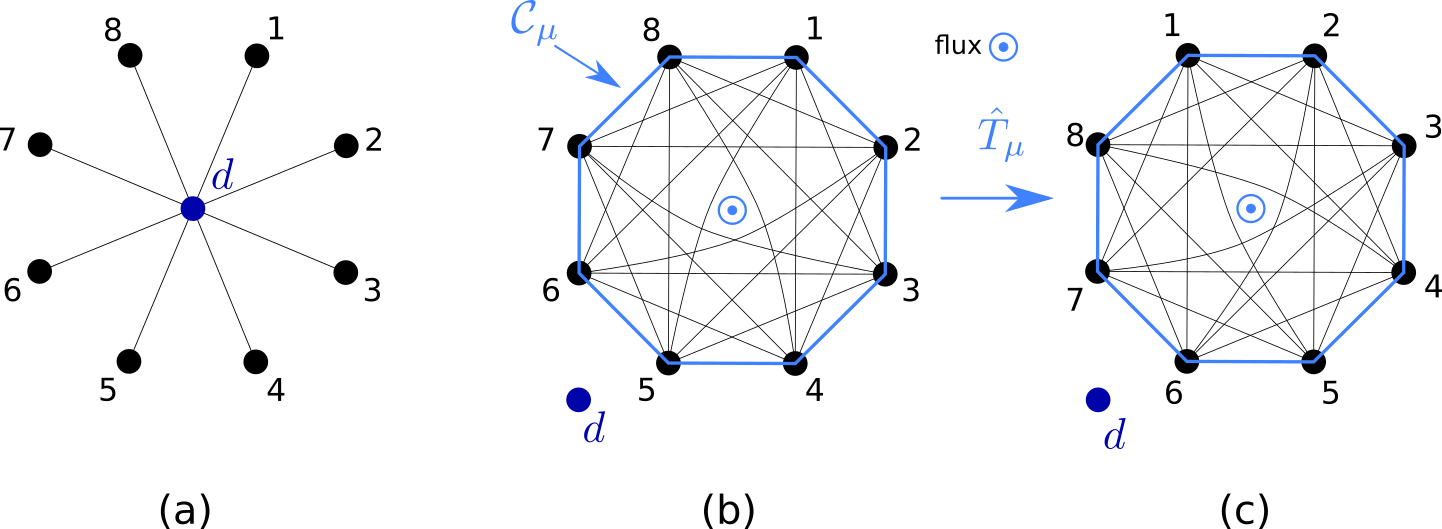
\includegraphics[scale=0.8]{plt/stargraph-to-alltoall}
\caption{This figure shows the comparison and mapping between the stargraph degenerate ground states and the states of the quantum fluctuation resolved all to all model.}
\label{fig:stargraph-to-alltoall}
\end{figure}
Thus one can see that the ground state degeneracy of the stargraph model with different $J^z$ values gets lifted in the quantum fluctuation resolved all-to-all model. Depending on the value of the flux there is an unique ground state labeled by the $J^z$ value. Tuning the fluc one can go from one ground state to the other. This shows how one can explore different degenerate ground states of the parent stargraph model via the insertion of flux in the corresponding quantum fluctuation resolved all-to-all effective Hamiltonian.



\subsection{Local mott-liquid}
Impurity-bath quantum fluctuation resolved all-to-all effective Hamiltonian is written in terms of the spinor spin operators which are individually made out of two electronic degree of freedom. This is defined as $\vec{S}_i=\frac{\hbar}{2} \displaystyle\sum_{\substack{ \alpha,\beta\in \{\uparrow,\downarrow\}}}  c_{0\alpha}^{(i)\dagger} \vec{\sigma}_{\alpha\beta} c_{0\beta}^{(i)}$. In the above eq.\eqref{eq:all-to-all_1} we see the $U(1)$ symmetry of the effective Hamiltonian. Using the spinor repersentation one can see the spin creation operation in terms of the electronic degree of freedom is 
\begin{eqnarray}
S_i^+ &=& \frac{\hbar}{2} \displaystyle\sum_{\alpha,\beta\in \{\uparrow\downarrow\}} c_{0\alpha}^{(i)\dagger} {\sigma}^{+}_{\alpha\beta} c_{0\beta}^{(i)}
% = \frac{\hbar}{2} \displaystyle\sum_{\alpha,\beta\in \{\uparrow\downarrow\}} c_{0\alpha}^{(i)\dagger}   c_{0\beta}^{(i)} \delta_{\uparrow,\alpha} \delta_{\downarrow,\beta} 
=\frac{\hbar}{2} c_{0\uparrow}^{(i)\dagger} c_{0\downarrow}^{(i)}  \\
S_i^z &=& \frac{\hbar}{2} \displaystyle\sum_{\alpha,\beta\in \{\uparrow\downarrow\}} c_{0\alpha}^{(i)\dagger} {\sigma}^{z}_{\alpha\beta} c_{0\beta}^{(i)} =\frac{\hbar}{2} (c_{0\uparrow}^{(i)\dagger} c_{0\uparrow}^{(i)} - c_{0\downarrow}^{(i)\dagger} c_{0\downarrow}^{(i)} )~,~~~~
\end{eqnarray}
Thus this spinor spins are nothing but the Anderson pseudospin formulation in the spin channel. The spin creation opertor ($S_i^+$) shows simultaneous creation of an electron-hole pair at the realspace origin of the $i^{th}$ channel. The condensation of such electron-hole pais has already been shown in [CITE: mott]. Thus for this effective Hamiltonian one can define twist-translation oeprations to construct the gauge theory and unveiling any hidden degeneracy. Let's recall the effective Hamiltonian
\begin{eqnarray}
H_{eff} &=& \frac{\beta_{\uparrow}(\alpha,\omega_{\uparrow})}{4} \bigg[ \displaystyle\sum_{ij} S_i^+S_j^- ~+ \textrm{h.c.} \bigg]~,
\end{eqnarray}
where $i,j$ are the channel indices. Due to the all-to-all nature of the connectivity one can draw total $K!$ possible unique closed paths ($\mathcal{C}_{\mu}$) where each nodes (channels) is being touched only once. One can thus define total $K!$ number of translation operators ($\hat{T}_{\mu}$) which keeps the Hamiltonian invariant. Let's define one of such translation operator $\hat{T}_{\mu}$ thich gives a periodic shifts along the closed path $\mathcal{C}_{\mu}$. Let's define twist operator along the path $\mathcal{C}_{\mu}$
\begin{eqnarray}
\hat{\mathcal{O}}_{\mu} &=& \exp({i\frac{2\pi}{K} \displaystyle\sum_{\substack{j=1\\ \mathcal{C}_{\mu}}}^{K} j S_j^z} )~,~~\hat{T}_{\mu}=e^{i\hat{P}^{cm}_{{\mu}}}
\end{eqnarray}
The  operation of the translation operator $\hat{T}_{\mu}$ is defined as $\hat{T}_{\mu} S_j^z = S_{j+1}^z$ where $j+1$ and $j$ are the nearest neighbor on the closed path $\mathcal{C}_{\mu}$. Then the braiding rule between the twist and translation operators are give as
\begin{eqnarray}
\hat{T}_{\mu}\hat{\mathcal{O}}_{\mu} \hat{T}^{\dagger}_{\mu} \hat{\mathcal{O}}_{\mu}^{\dagger}  &=&  \exp\{i[2\pi S_1^z-\frac{2\pi}{K}S^z]\} \nonumber\\
&=& \exp\{i[\pm \pi - \frac{2\pi}{K} S^z]\} =\exp(i\frac{2\pi p}{q})
\end{eqnarray}
The availability of the non-trivial braiding staatistics between these twist and translation operators is possible if $p\neq 0$ and $q\neq \infty$. Further simplification leads to the condition
\begin{eqnarray}
 \pm\pi -\frac{2\pi}{K} S^z = \frac{2\pi p}{q} ~~ &\Rightarrow & \pm\frac{1}{2}-\frac{S^z}{K} = \frac{p}{q} \nonumber\\
&& \frac{(\pm K-2S^z)}{2K} = \frac{p}{q}~,~
\end{eqnarray} 
$p,q$ are mutual prime, We knwo that the $S^z$ can take values $(\mp K/2\pm m)$ where $m$ is a integer $0 \leq m \leq K$. Putting this value in the above equation leads to two possible solutions.
\begin{eqnarray}
\frac{(K-m)}{K} &=& \frac{p}{q} ~,~~ \frac{-m}{K}=\frac{p}{q}
\end{eqnarray}
For the first case $K-m=p$ we can see that $m=K$ makes $p$ trivial hus the allowed values are $m=0,\cdots,K-1$, which represents the corresponding $S^z$ eigen values 
\begin{eqnarray}
&&-K/2,-K/2+1,\cdots,K/2-2,K/2-1
\end{eqnarray}
Similarly the second case implies, $-m=p$, but $p=0$ is not allowed as this makes the braiding statistics trivial, thus the possible $S^z$ values are 
\begin{eqnarray}
&&\hspace{2.2cm} -K/2+1,-K/2+2,\cdots,K/2-1,K/2
\end{eqnarray}

\noindent Thus we get the general braiding statistics between the twist and the translation 
\begin{eqnarray}
\hat{T}_{\mu}\hat{\mathcal{O}_{\mu}} \hat{T}^{\dagger}_{\mu}\hat{\mathcal{O}_{\mu}}^{\dagger} &=& e^{i\frac{2\pi p}{K}}
\end{eqnarray}
where $p$ corresponds to different $S^z$ states, related as $p=\pm K/2-S^z$. Thus we can see that there are $K$ possible $S^z$ plaleau states in the all-to-all model where each plateaux is $K$ fold degenerate. This $p/K$ is similar to the filling factor of the fractional quantum Hall effect. There are possibly $K!$ pairs of twist and translation operator corresponding to different closed paths $\mathcal{C}_{\mu}$ which can probe this degeneracy.

\subsubsection{Action on the Hamiltonian}
Now we findout the action of these twist operators on the Hamiltonian. The Hamiltonian is written as 
\begin{eqnarray}
H_{eff}&=& \frac{\beta_{\uparrow}(\alpha,\omega_{\uparrow})}{2} (S^{x2} +S^{y2})   
\end{eqnarray}
Due the all-to-all nature of the effetive Hamiltonian one can find $K!$ possible relative arrangement of those $K$ channels which keeps the Hamiltonian invariant. Here we briefly discuss the choice of the closed loop $\mathcal{C}_{\mu}$ and the insertion of the flux. As shown in the Fig.\ref{fig:stargraph-to-alltoall}(b) we have chosen a particular closed path which crosses all the outer spin only once. We embed that closed loop on a plane and put the flux perpendiculr to the plane through the closed loop. One can find a different closed loop where the ordering of the outer spins will be different. The action of the translation operator shifts the outer spins along this closed curve by one step.

The action of the twist operator on the $S^x$ is determined in the follwoing calculation
%\begin{eqnarray}
%\hat{O}_{\mu} S^x \hat{O}^{\dagger}_{\mu} &=& \exp({i\frac{2\pi}{K} \displaystyle\sum_{\substack{j=1\\ \mathcal{P}_{\mu}}}^{K} j S_j^z} ) ~~S^x ~~ \exp({-i\frac{2\pi}{K} \displaystyle\sum_{\substack{j=1\\ \mathcal{P}_{\mu}}}^{K} j S_j^z} )= e^{X} S^x e^{-X} \nonumber\\
%&=& S^x+[X,S^x] + \frac{1}{2!}[X,[X,S^x]] +\cdots  
%\end{eqnarray}
%For simplicity of thte calculation we define $i\frac{2\pi}{K}=\Omega$, thus $X=\Omega\sum_j jS^z_j$.
%\begin{eqnarray}
%&& [X,S^x] = [\Omega\sum_j jS^z_j,\sum_{l} S^x_l] =\Omega \sum_j j[S^z_j,S^x_j] = (i\Omega) \sum_j j S^y_j \nonumber\\
%&& [X,S^y] = [\Omega\sum_j jS^z_j,\sum_{l} S^y_l] =\Omega \sum_j j[S^z_j,S^y_j] = -(i\Omega) \sum_j j S^x_j  \nonumber\\
%&& [X,[X,S^x]] = [X,i\Omega \sum_j j S^y_j] = [\Omega\sum_{l}l S_l^z,i\Omega \sum_j j S^y_j] =i\Omega^2\sum_{l} l^2[ S_l^z, S^y_j] =-(i^2\Omega^2)\sum_{l} l^2 S_l^x ~,~~~~ \nonumber\\
%&& [X,[X,S^y]] = [X,-i\Omega \sum_j j S^x_j] = [\Omega\sum_{l}l S_l^z,-i\Omega \sum_j j S^x_j] =-i\Omega^2\sum_{l} l^2[ S_l^z, S^x_j] =-(i^2\Omega^2)\sum_{l} l^2 S_l^y ~,~~~~~~~~ \nonumber\\
%&& [X, [X,[X,S^x]]] = [\Omega\sum_j jS^z_j,-i^2\Omega^2 \sum_l l^2 S_l^x ]=-i^2\Omega^3 \sum_l l^3[S^z_l,S^x_l] =-(i^3\Omega^3) \sum_l l^3 S^y_l  \nonumber\\
%&& [X, [X,[X,S^y]]] = [\Omega\sum_j jS^z_j,-i^2\Omega^2 \sum_l l^2 S_l^y ]=-i^2\Omega^3 \sum_l l^3[S^z_l,S^y_l] =(i^3\Omega^3) \sum_l l^3 S^x_l 
%\end{eqnarray}
%Thus we get
%\begin{eqnarray}
%e^X S^x e^{-X}&=& S^x+[X,S^x] + \frac{1}{2!}[X,[X,S^x]] +\cdots  \nonumber\\
%&=& \sum_l S_l^x + (i\Omega)\sum_l l S^y_l + \frac{-(i\Omega)^2}{2!}\sum_{l} l^2 S_l^x + \frac{-(i\Omega)^3}{3!} \sum_l l^3 S_l^y+ \cdots \nonumber\\
%&=& \sum_l S_l^x \bigg[1-\frac{(il\Omega)^2}{2!}  +\cdots \bigg] + \sum_{l} S_l^y \bigg[ (il\Omega)- \frac{(il\Omega)^3}{3!} +\cdots \bigg] \nonumber\\
%&=& \sum_l \bigg[ S^x_l \cos (il\Omega) +  S_l^y \sin(il\Omega) \bigg] =  \sum_l \bigg[ S^x_l \cos (-\frac{2\pi l}{K}) +  S_l^y \sin(-\frac{2\pi l}{K}) \bigg]  \nonumber\\
%&=& \sum_l ( S^x_l \cos \theta_l -  S_l^y \sin \theta_l ) ~,~~~\theta_l=\frac{2\pi l}{K}
%\end{eqnarray}
%
%\begin{eqnarray}
%e^X S^y e^{-X}&=& S^y+[X,S^y] + \frac{1}{2!}[X,[X,S^y]] +\cdots  \nonumber\\
%&=& \sum_l S_l^y - (i\Omega)\sum_l l S^x_l + \frac{-(i\Omega)^2}{2!}\sum_{l} l^2 S_l^y + \frac{(i\Omega)^3}{3!} \sum_l l^3 S_l^x+ \cdots \nonumber\\
%&=& \sum_l S^y_l \bigg[ 1 -\frac{(il\Omega)^2}{2!} + \cdots \bigg]- \sum_l S^x_l \bigg[ (il\Omega) - \frac{(il\Omega)^3}{3!} +\cdots \bigg] \nonumber\\
%&=& \sum_l  (S^y_l \cos\theta_l  + S^x_l \sin\theta_l)
%\end{eqnarray}
%As already defined, $\theta_l=\frac{2\pi l}{K}=\frac{2\pi (K-n)}{K}$, where $n$ is an integer. We can see that in the large channel limit $\theta_l $ becomes inter multiple of $2\pi$. Thus in the large channel limit
%
%%\begin{eqnarray}
%%\hat{\mathcal{O}}_{\mu} S^{\nu} \hat{\mathcal{O}}^{\dagger}_{\mu} &\xRightarrow[]{K \rightarrow \infty } S^{\nu}~,~~\nu=x,y 
%%\end{eqnarray}
%
%\textbf{\textit{Fix this LaTeX issue (equation)}}

Thus in the large channel limit
\begin{eqnarray}
&& \lim_{K\rightarrow \infty}\hat{\mathcal{O}}_{\mu} H_{eff} \hat{\mathcal{O}}_{\mu}^{\dagger}\nonumber\\
 &=& \frac{\beta_{\uparrow}(\alpha,\omega_{\uparrow})}{2} \bigg[ \hat{\mathcal{O}}_{\mu} S^x \hat{\mathcal{O}}_{\mu}^{\dagger} \hat{\mathcal{O}}_{\mu} S^x \hat{\mathcal{O}}_{\mu}^{\dagger}  + \hat{\mathcal{O}}_{\mu} S^y \hat{\mathcal{O}}_{\mu}^{\dagger} \hat{\mathcal{O}}_{\mu} S^y \hat{\mathcal{O}}_{\mu}^{\dagger}  \bigg]\nonumber\\
&=&\frac{\beta_{\uparrow}(\alpha,\omega_{\uparrow})}{2} \bigg[  S^{x2}+S^{y2}  \bigg] = H_{eff} \nonumber\\
&&\lim_{K\rightarrow \infty } [\hat{\mathcal{O}},H_{eff}] = 0
\label{eq:hamiltonian_twisted}
\end{eqnarray}
 
\noindent The translation operator $\hat{T}_{\mu}=e^{i\hat{\mathcal{P}}_{\mu}}$ commutes with the Hamiltonian thus the generator $\hat{\mathcal{P}}_{\mu}$ also commutes with the Hamiltonian. We can label the $j^{th}$ state with the eigenvalues of this operator $\hat{\mathcal{P}_{\mu}}$ as $|p^{j}_{\mu}\rangle$. We here discuss the action of these twist and translation operators on these states.
\begin{eqnarray}
\hat{T}_{\mu} |p^j_{\mu} \rangle &=& e^{i\hat{\mathcal{P}}_{\mu}} |p^j_{\mu} \rangle = e^{ip^j_{\mu}} |p^j_{\mu}\rangle \nonumber\\
\hat{T}_{\mu} \hat{\mathcal{O}}_{\mu} |p^j_{\mu} \rangle &=&  \hat{\mathcal{O}}_{\mu} \hat{T}_{\mu} e^{i\frac{2\pi m}{K}} |p^j_{\mu}\rangle~~, \nonumber\\
&&~~\textrm{here $m$ signifies different $S^z$ plateaux.} \nonumber\\ \nonumber\\
&=& \hat{\mathcal{O}}_{\mu}   e^{i(\frac{2\pi m}{K}+p_{\mu}^j)} |p^j_{\mu}\rangle~,~~ \frac{2\pi m}{K} \equiv p_{\mu}^{m} \nonumber\\
\hat{T}_{\mu} \bigg( \hat{\mathcal{O}}_{\mu} |p^j_{\mu} \rangle  \bigg) &=& e^{i(p_{\mu}^{m}+p_{\mu}^j)} \bigg( \hat{\mathcal{O}}_{\mu}    |p^j_{\mu}\rangle \bigg)    
\end{eqnarray}
Thus we can see that  $\hat{\mathcal{O}}_{\mu} |p^j_{\mu} \rangle $ is a state of the traslation operator with different eiven value than $|p^j_{\mu} \rangle $, thus orthogonal to each other. Simiarly one can generally show that $\langle p^j_{\mu} | \hat{\mathcal{O}}^{q}_{\mu} |p^j_{\mu} \rangle=0$, where $q$ is any integer. Also in the large $K$ limit we can see from the eq.\eqref{eq:hamiltonian_twisted} that these differnt twisted states has same energy. Which shows that at each plateau state labeled by the $S^z$ eigenvalue has $K$ fold degenerate eigenstates labeled by the eigenvalue of the translation operators. Thus the CSCO is formed by $H,S^z,\hat{T}$. Thus states can be lebeled as  $|E,S^z_j,P^j_{\mu}\rangle$. 







\end{document}